\chapter{Resultados}
\label{chapter:resultados}

La validación de una implementación computacional constituye un proceso esencial que va más allá de la simple verificación de que el código ejecuta sin errores. En el contexto de modelos neuronales complejos como el de \citet{echeveste2020cortical}, la correctitud de la implementación debe evaluarse en múltiples niveles, desde la precisión numérica de funciones individuales hasta la emergencia de propiedades dinámicas globales que definen el comportamiento del sistema.

Este capítulo presenta los resultados de un proceso de validación estructurado en cuatro niveles complementarios. En primer lugar, se describe la infraestructura de \textbf{pruebas automatizadas} desarrollada para verificar componentes individuales del modelo. En segundo lugar, se presenta una \textbf{validación función por función} que compara directamente nuestra implementación con el código original de Echeveste, demostrando equivalencia numérica a nivel de precisión de punto flotante. En tercer lugar, se analizan los resultados del \textbf{procedimiento de entrenamiento}, comparando los parámetros optimizados con los valores de referencia. Finalmente, se presentan \textbf{simulaciones comparativas} que replican las figuras centrales del artículo original, demostrando que la red implementada exhibe las propiedades de inferencia probabilística características del modelo.

% =============================================================================
% SECCIÓN 1: INFRAESTRUCTURA DE VALIDACIÓN
% =============================================================================

\section{Infraestructura de validación}
\label{sec:res_tests}

La validación de una reimplementación completa (desde OCaml hacia Python/JAX) requiere verificar no solo que los componentes individuales funcionen correctamente de manera aislada, sino también que su comportamiento numérico sea idéntico al del código de referencia. Esta sección describe la infraestructura de pruebas automatizadas desarrollada para garantizar la fidelidad de la implementación, organizada en pruebas unitarias que verifican la lógica interna y pruebas de integración que evalúan la equivalencia con el código original.

\subsection{Pruebas unitarias de la clase principal}
\label{subsec:res_tests_main}

El archivo \texttt{test\_echeveste2020.py} implementa once clases de pruebas que cubren los aspectos fundamentales del modelo. Estas verificaciones aseguran la correcta inicialización con parámetros por defecto y personalizados, permitiendo que el modelo se instancie con diferentes tamaños de red y constantes de tiempo sin generar errores.

Un aspecto crítico es la verificación de la \textbf{matriz de conectividad}. Las pruebas comprueban que la matriz $\mathbf{W}$ tenga la forma correcta, que respete el principio de Dale, y que exhiba la topología de anillo esperada según la Ecuación~\ref{eq:weight_parametrization}. Específicamente, se verifica que los bloques $\mathbf{W}_{EE}$ y $\mathbf{W}_{IE}$ contengan únicamente valores positivos, que los bloques $\mathbf{W}_{EI}$ y $\mathbf{W}_{II}$ contengan únicamente valores negativos, y que cada bloque exhiba estructura circulante donde $W_{ij}$ depende únicamente de $|\theta_i - \theta_j|$.

La \textbf{función de activación supralineal} (Ecuación~\ref{eq:firing_rate}) se prueba exhaustivamente para garantizar el comportamiento correcto:
\begin{equation} \notag
r = k \cdot [u]_+^n = 0.3 \cdot [\max(0, u)]^2
\label{eq:firing_rate_test}
\end{equation}
Las pruebas verifican el comportamiento para potenciales negativos (tasa cero), potenciales positivos (respuesta cuadrática), y casos límite. Esta verificación resulta fundamental dado que cualquier error en la función de transferencia se propagaría a través de toda la dinámica de la red.

\subsection{Pruebas unitarias del módulo de entrenamiento}
\label{subsec:res_tests_training}

A su vez, el archivo \texttt{test\_echeveste2020\_training.py} también implementa pruebas específicas para el procedimiento de optimización en dos etapas descrito en la Sección~\ref{sec:impl_entrenamiento}. Estas pruebas son particularmente delicadas dado que el entrenamiento involucra diferenciación automática a través de ecuaciones diferenciales estocásticas.

Las pruebas verifican que los 8 parámetros de conectividad ($a_{EE}$, $a_{EI}$, $a_{IE}$, $a_{II}$, $d_{EE}$, $d_{EI}$, $d_{IE}$, $d_{II}$) se actualizan correctamente durante la optimización, que las restricciones de bounds se respetan (amplitudes $\geq 0$, anchos $\in [0, \sqrt{2}]$), y que la función de costo decrece monótonamente a lo largo de las iteraciones. A su vez, se verifica la construcción correcta de la matriz de covarianza de ruido $\boldsymbol{\Sigma}_\eta$, incluyendo su dimensión, simetría, positividad semi-definida, y estructura de bloques consistente con las Ecuaciones~\ref{eq:noise_cov_same} y \ref{eq:noise_cov_cross}.

Las pruebas end-to-end verifican que el método \texttt{train()} complete ambas etapas sin errores y que la red entrenada pueda ejecutar simulaciones estables sin divergir numéricamente.

% \subsection{Pruebas de componentes de integración}
% \label{subsec:res_tests_integration}

% Finalmente implementamos comparaciones directas entre nuestra implementación y los datos generados por el código original de \citeauthor{echeveste2020cortical}, disponible en su repositorio de referencia. Estas pruebas constituyen la validación más rigurosa, ya que verifican la equivalencia numérica punto por punto.

% Las comparaciones incluyen:

% \textbf{Filtros de Gabor:} Se verifica que la matriz $\mathbf{A}$ generada por nuestra implementación coincida con los filtros almacenados en el repositorio original. El criterio de aceptación requiere una correlación de Pearson superior a 0.95 entre cada par de filtros correspondientes.

% \textbf{Matriz de covarianza \textit{a priori}:} La matriz $\mathbf{C}$ del modelo generativo \acrshort{GSM} debe reproducir la estructura circular de correlaciones con correlación superior a 0.7 respecto al archivo de referencia.

% \textbf{Transformación de entrada $\mathbf{h}$:} Para estímulos de prueba idénticos, la entrada feedforward calculada según la Ecuación~\ref{eq:feedforward_input} debe coincidir con tolerancia $\text{MSE} < 10^{-10}$.

% \textbf{Pipeline completo:} La secuencia filtros $\rightarrow$ covarianza $\rightarrow$ transformación debe alcanzar correlaciones superiores a 0.99 para filtros y 0.95 para la matriz de covarianza.

% \begin{table}[H]
% \centering
% \caption{Resumen de pruebas de integración con código original.}
% \label{tab:test_summary}
% \begin{tabular}{lcc}
% \toprule
% \textbf{Componente} & \textbf{Métrica} & \textbf{Resultado} \\
% \midrule
% Filtros de Gabor & Correlación & $> 0.99$ \\
% Covarianza \textit{a priori} & Correlación & $> 0.95$ \\
% Transformación $\mathbf{h}$ & \acrshort{MSE} & $< 10^{-10}$ \\
% Matriz de conectividad $\mathbf{W}$ & Diferencia máxima & $< 10^{-8}$ \\
% Parámetros cargados & Tolerancia & $< 10^{-6}$ \\
% \bottomrule
% \end{tabular}
% \end{table}

% Todas estas pruebas se ejecutan automáticamente como parte del proceso de integración continua del proyecto, garantizando que cualquier modificación al código que introduzca regresiones sea detectada inmediatamente.

\subsection{Validación función por función contra código original}
\label{subsec:res_function_validation}

Más allá de las pruebas unitarias que verifican la lógica interna, se realizó una validación exhaustiva comparando cada función de nuestra implementación con su equivalente en el código original de \citeauthor{echeveste2020cortical}. Este proceso constituye la verificación más rigurosa de equivalencia numérica, ya que evalúa directamente si ambas implementaciones producen resultados idénticos para los mismos inputs.

La metodología consistió en generar $N = 10{,}000$ muestras aleatorias para cada función, ejecutar tanto la implementación original como la nuestra con inputs idénticos, y calcular el error máximo absoluto entre los resultados. Las funciones se organizaron en ocho categorías que cubren todos los componentes matemáticos del modelo, desde funciones auxiliares básicas hasta el cálculo completo de la posterior del \acrshort{GSM}.

La Tabla~\ref{tab:function_validation_summary} presenta el resumen de esta validación por categoría. Los resultados demuestran que todas las 25 funciones evaluadas producen resultados numéricamente equivalentes, con errores máximos del orden de la precisión de punto flotante de doble precisión ($\sim 10^{-15}$ a $10^{-16}$).

\begin{table}[H]
\centering
\caption{Resumen de validación función por función contra código original de Echeveste ($N = 10\,000$ muestras por función).}
\label{tab:function_validation_summary}
\makebox[\textwidth][c]{
\begin{tabular}{clcc}
\toprule
\textbf{\#} & \textbf{Categoría} & \textbf{Error máximo} & \textbf{Estado} \\
\midrule
1 & Distribución Normal (\texttt{f1}, \texttt{f2\_exact}) & $0.00$ & \checkmark \\
2 & Activación Neuronal (\texttt{get\_r}, \texttt{get\_r\_prime}) & $0.00$ & \checkmark \\
3 & Momentos $\nu$, $\gamma$ (\texttt{nu\_recursive}, \texttt{get\_gamma}) & $7.11 \times 10^{-15}$ & \checkmark \\
4 & Evolución Temporal (\texttt{new\_u}, \texttt{mu\_dot}, \texttt{u\_dot\_det}) & $0.00$ & \checkmark \\
5 & Conectividad Paramétrica (kernel Eq.~\ref{eq:weight_parametrization}, \texttt{get\_J}) & $0.00$ & \checkmark \\
6 & Ruido O-U (\texttt{eps\_1}, \texttt{eps\_2}, update step) & $1.11 \times 10^{-16}$ & \checkmark \\
7 & GSM Posterior ($\Sigma_z$, $\mu_z$, \texttt{get\_x}, $P_z$) & $0.00$ & \checkmark \\
8 & Funciones Auxiliares (\texttt{sqr\_norm}, \texttt{rel\_error}, etc.) & $0.00$ & \checkmark \\
\bottomrule
\end{tabular}
}
\end{table}

Los errores no nulos observados en las categorías 3 y 6 corresponden exactamente a la precisión de punto flotante IEEE 754 de doble precisión, donde el épsilon de máquina es $\epsilon \approx 2.22 \times 10^{-16}$. Estos errores surgen de diferencias en el orden de operaciones aritméticas entre implementaciones y no representan discrepancias algorítmicas.

La Figura~\ref{fig:function-validation-complete} en el Apéndice~\ref{appendix:validation} presenta el detalle completo de las 25 funciones validadas, incluyendo las referencias a las líneas de código específicas tanto en el repositorio original como en nuestra implementación. Esta trazabilidad permite verificar independientemente la correspondencia entre ambas bases de código.

Estos resultados proporcionan confianza de que cualquier diferencia observada en el comportamiento de alto nivel del modelo (dinámicas, propiedades de muestreo) no puede atribuirse a errores en la implementación de funciones individuales.

\subsection{Consistencia en la generación de estímulos}
\label{subsec:res_tests_gsm_stimuli}

Un requisito fundamental para las siguientes validaciones, es asegurar que el modelo generativo \acrshort{GSM} implementado en \textit{Scikit-NeuroMSI} genere estímulos idénticos a los del código original bajo las mismas configuraciones. Para ello, se verificó la consistencia del vector de entrada $\mathbf{h}$ a través de cuatro variantes del pipeline de generación, comparando los resultados con los datos precomputados de referencia.

Como se observa en la Figura~\ref{fig:gsm_comparison}, se evaluaron los siguientes flujos de datos:

\begin{itemize}
    \item \textbf{h\_true (precomputed):} Valores de $\mathbf{h}$ extraídos directamente de los archivos \texttt{.mat} originales, son los datos reales utilizados por \citeauthor{echeveste2020cortical} en la simulación representando el objetivo numérico a replicar.
    \item \textbf{GSM loaded stimulus:} El vector $\mathbf{h}$ generado por nuestra implementación utilizando el estímulo sensorial $\mathbf{x}$ cargado de los archivos originales ($\mathbf{x}_{\text{loaded}} \rightarrow \mathbf{h}$).
    \item \textbf{GSM from y\_latent:} Un paso antes, recuperando solo el vector latente $\mathbf{y}$ se resuelve el sistema lineal $\mathbf{x} = z\mathbf{A}\mathbf{y}$ a partir de los datos originales, y luego se regenera $\mathbf{x}$ y $\mathbf{h}$ desde dicho $\mathbf{y}$.
    \item \textbf{GSM bump:} Generación sintética completa mediante nuestra función \texttt{generate\_bump\_stimulus(A, $\sigma$)}, utilizando una amplitud de 6.0 y un factor de ancho de 0.15, sin recurrir a datos externos.
\end{itemize}

\begin{figure}[H]
    \centering
    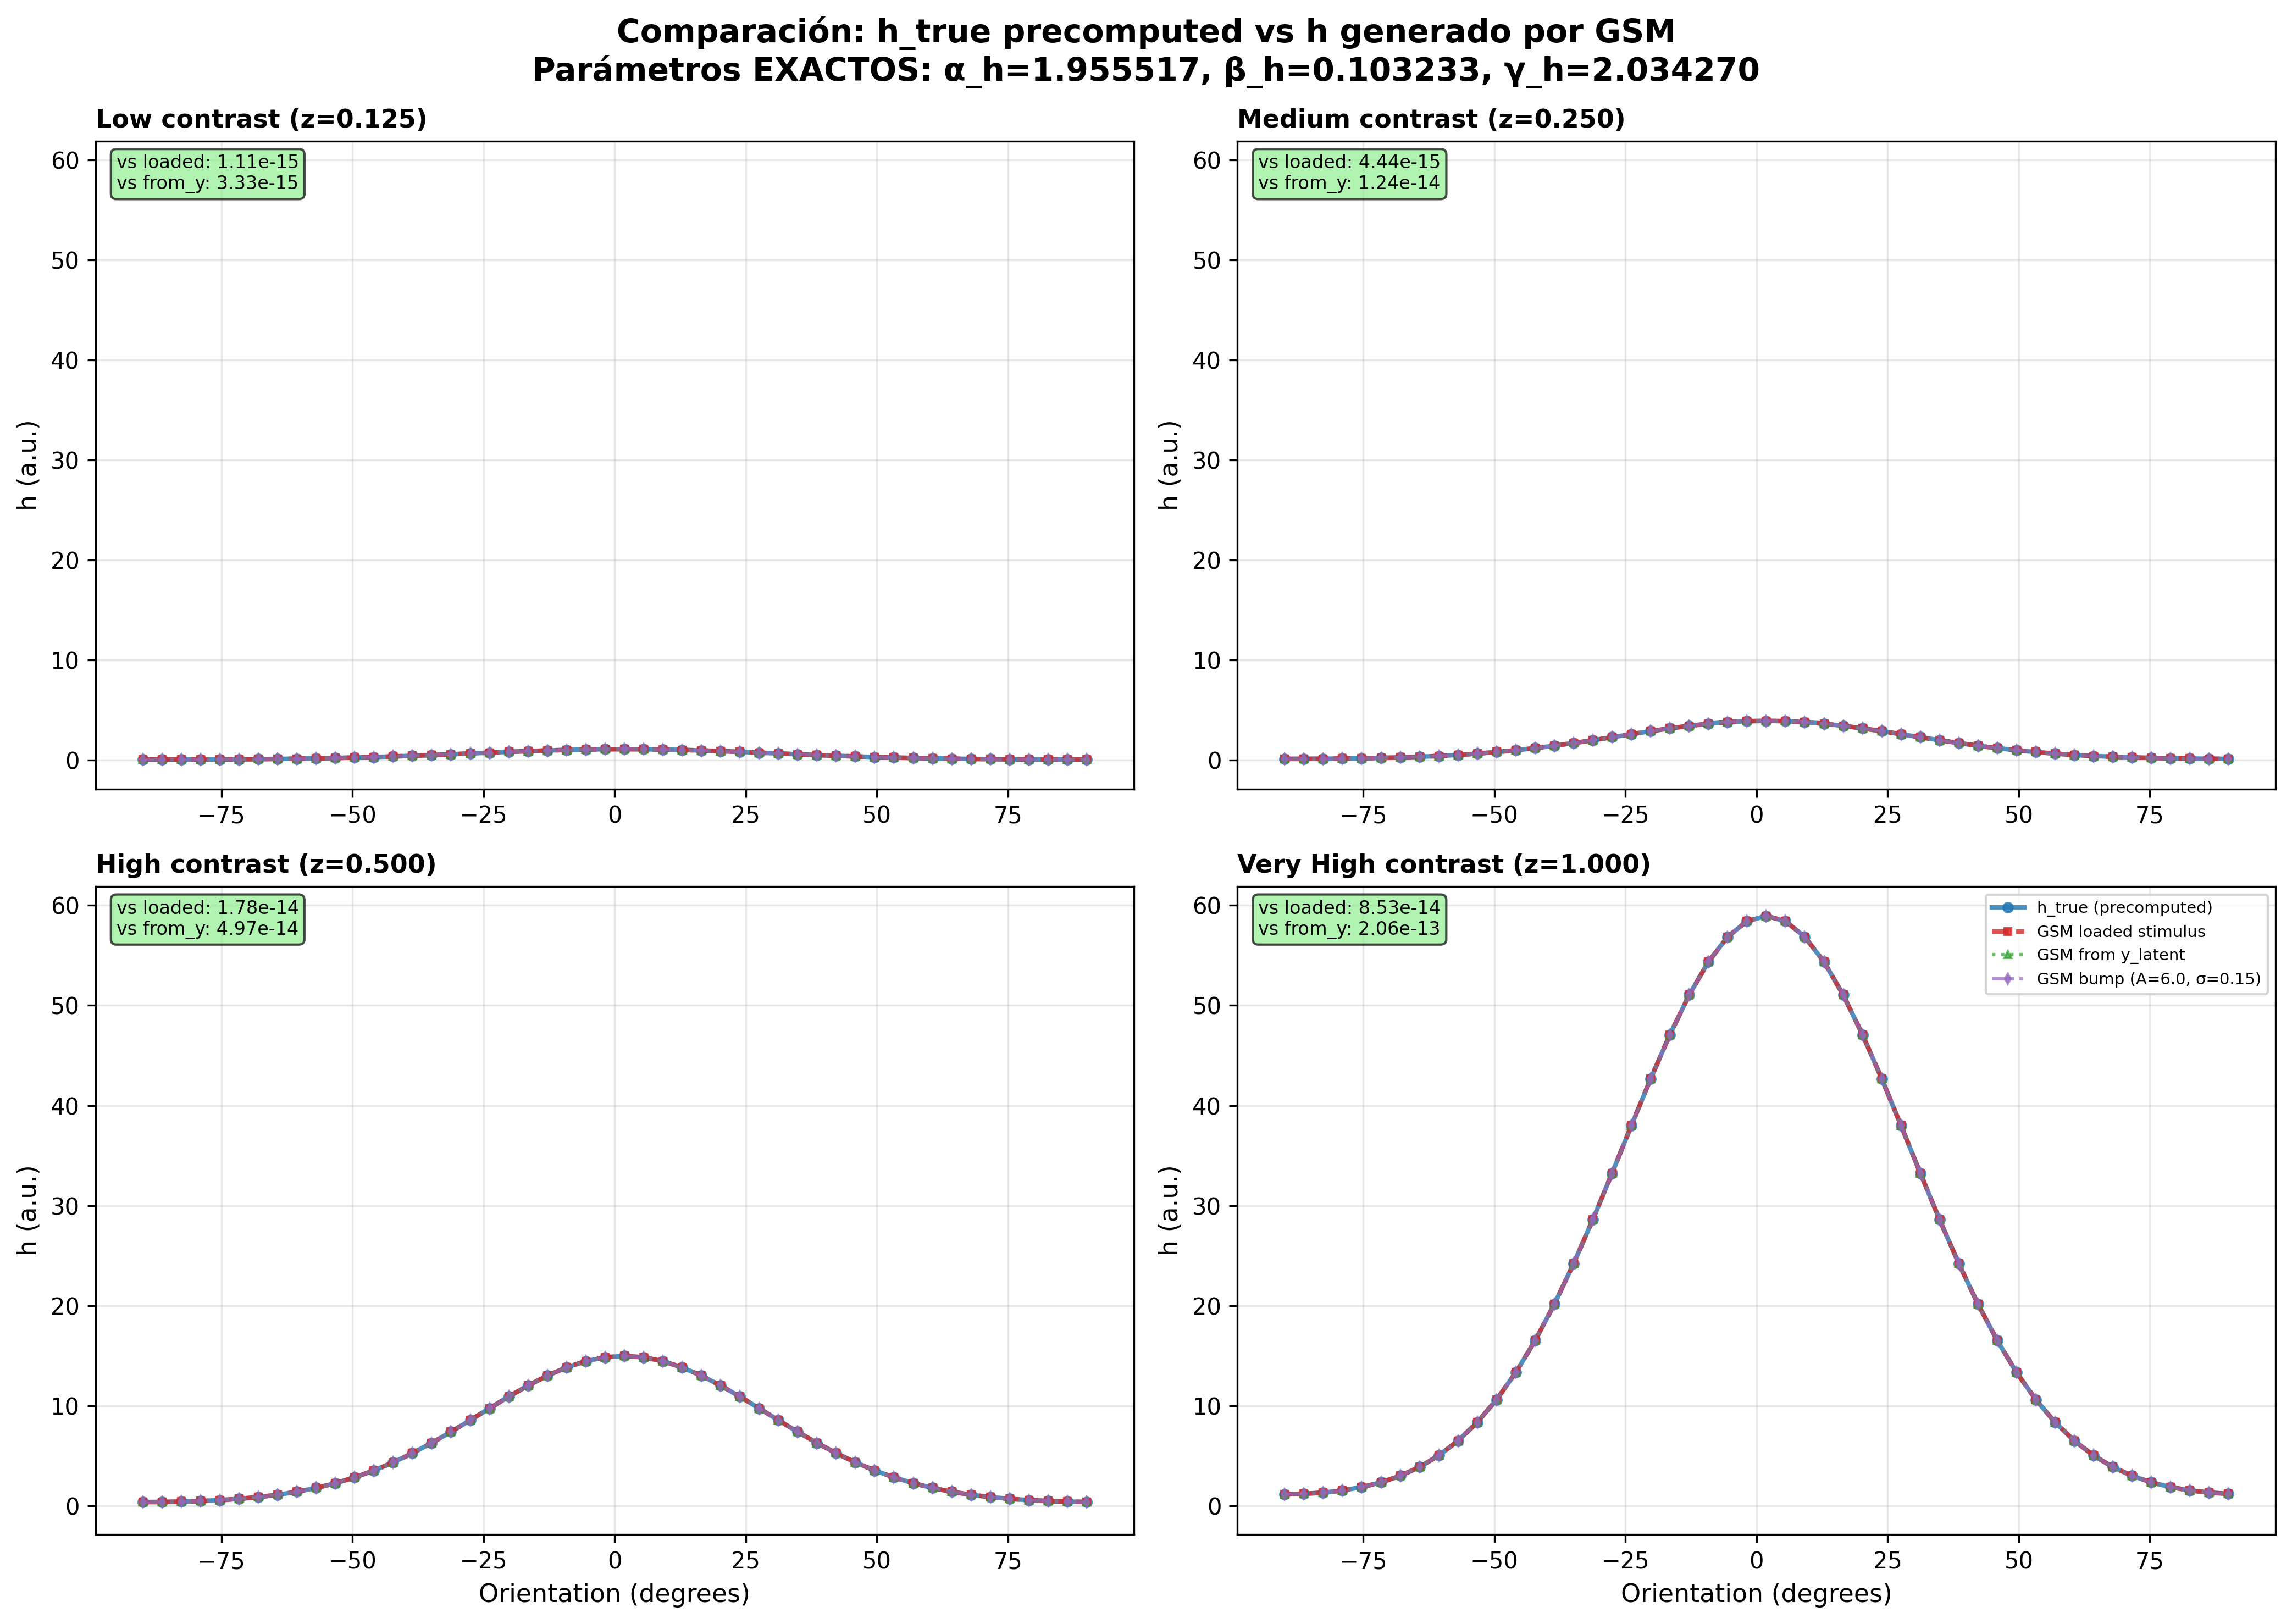
\includegraphics[width=1\textwidth]{08_resultados/figures/comparaciones_gsm_h.png}
    \caption{Comparación de la entrada $\mathbf{h}$ generada por el \acrshort{GSM} frente a los datos de referencia de Echeveste. Los paneles muestran cuatro niveles de contraste ($z$). La coincidencia entre las curvas (\acrshort{MSE} $< 10^{-13}$) confirma que el pipeline de generación y la transformación no lineal son idénticos a la implementación de referencia.}
    \label{fig:gsm_comparison}
\end{figure}

Los resultados muestran diferencias del orden de $10^{-13}$ a $10^{-15}$, garantizando que cualquier discrepancia posterior en la dinámica de la red no se deba a errores en la generación del estímulo de entrada. 

% =============================================================================
% SECCIÓN 2: VALIDACIÓN DEL ENTRENAMIENTO
% =============================================================================

\section{Validación del procedimiento de entrenamiento}
\label{sec:res_training}

Una vez verificada la equivalencia numérica de los componentes individuales, el siguiente nivel de validación consiste en confirmar que el procedimiento de entrenamiento converge hacia parámetros comparables a los reportados por \citet{echeveste2020cortical}. Esta validación resulta particularmente significativa dado que nuestra implementación en JAX\footnote{\url{https://docs.jax.dev/}} constituye una reimplementación completa del código original en OCaml\footnote{\url{https://ocaml.org/}}, como se describió en la Sección~\ref{subsec:impl_jax}.

\subsection{Diseño del experimento}
\label{subsec:res_training_design}

Para evaluar la robustez del procedimiento de entrenamiento, se ejecutaron múltiples corridas independientes partiendo de condiciones iniciales aleatorias. Cada corrida siguió el protocolo de dos etapas descrito en la Sección~\ref{sec:impl_entrenamiento}: Stage 1 con 250 iteraciones de \acrshort{ADAM} ($\eta = 0.002$, $N_{\text{trial}} = 50$), seguido de Stage 2 con optimización \acrshort{L-BFGS-B} utilizando el método \acrshort{ADF} para gradientes determinísticos.

Los valores de referencia corresponden a los parámetros optimizados reportados en la Tabla Suplementaria S1 del artículo original, reproducidos en la Tabla~\ref{tab:parametros_completos} del Capítulo~\ref{chapter:implementacion}.

\subsection{Convergencia de parámetros de conectividad}
\label{subsec:res_training_connectivity}

La Figura~\ref{fig:connectivity_results} presenta los resultados de la optimización para los parámetros de conectividad. En cada panel, los puntos representan los valores obtenidos en corridas individuales, la línea punteada roja indica el valor de referencia de Echeveste, y la banda sombreada corresponde a una tolerancia de $\pm 10\%$.

\begin{figure}[!ht]
    \centering
    \makebox[\textwidth][c]{%
        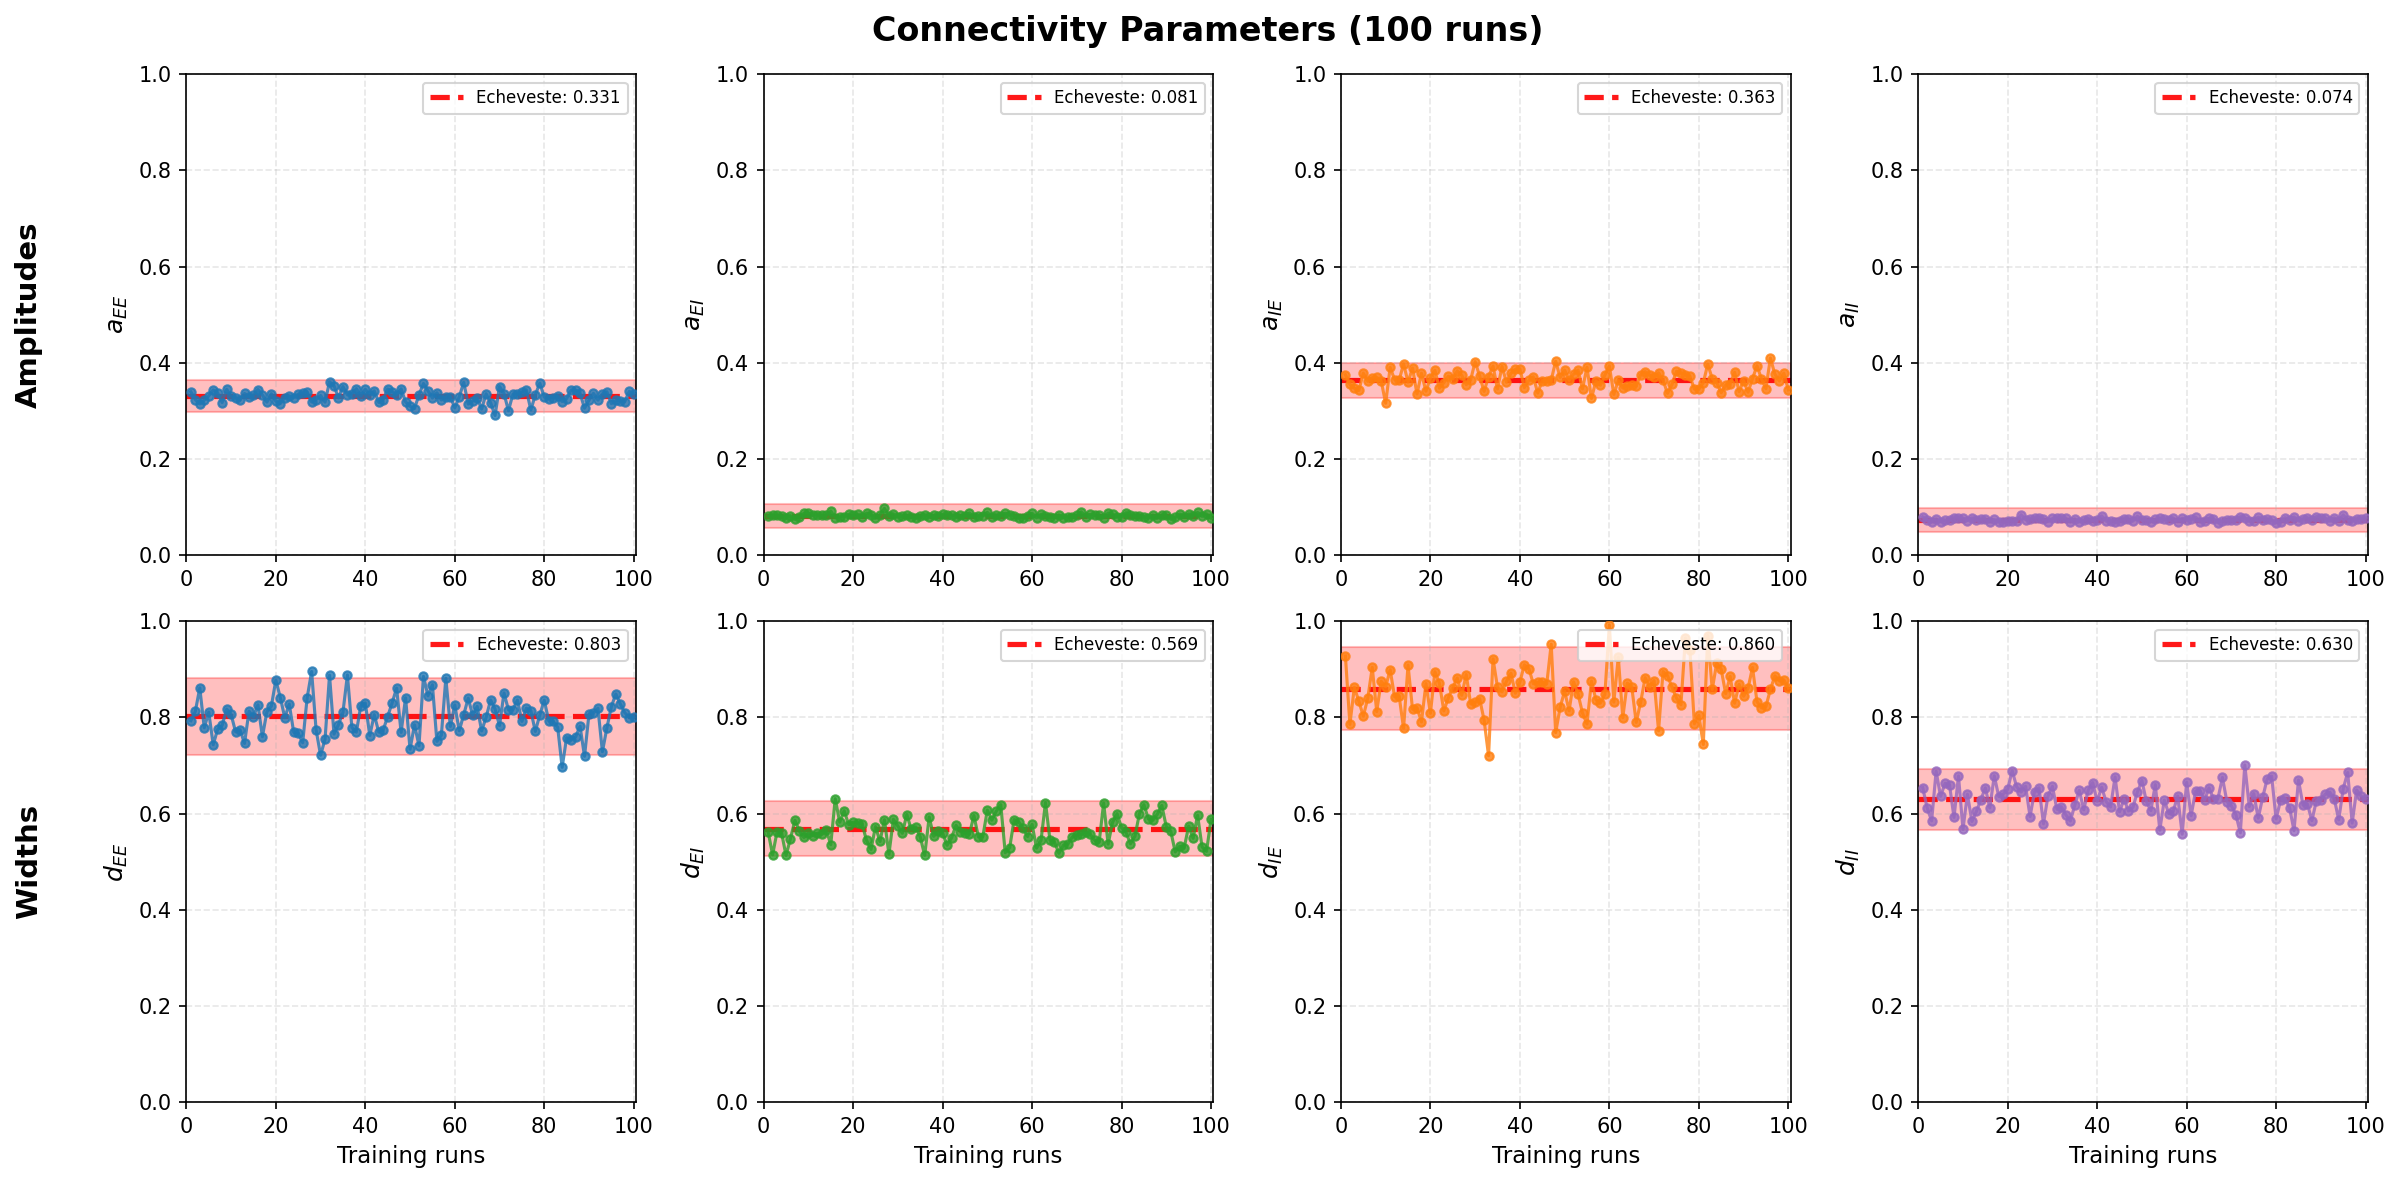
\includegraphics[width=1.25\textwidth]{08_resultados/figures/connectivity_results.png}
    }
    \caption{Parámetros de conectividad optimizados en 100 corridas independientes.}
    \label{fig:connectivity_results}
\end{figure}


Los resultados muestran que las amplitudes de conectividad convergen consistentemente hacia valores cercanos a los de referencia, como se detalla en la Tabla~\ref{tab:connectivity_amplitudes}. Las amplitudes exhiben baja variabilidad entre corridas (coeficientes de variación $< 0,1$), indicando que el paisaje de optimización tiene una estructura bien definida para estos parámetros.

\begin{table}[H]
\centering
\caption{Convergencia de amplitudes y anchos de conectividad ($N = 100$ corridas independientes). El coeficiente de variación (CV) se expresa como el cociente entre la desviación estándar y la media.}
\label{tab:connectivity_amplitudes}
\begin{tabular}{lcccc}
\toprule
\textbf{Parámetro} & \textbf{Referencia} & \textbf{Obtenido} & \textbf{CV} & \textbf{Tolerancia} \\
\midrule
% $a_{EE}$ & 0.331 & $0.34 \pm 0.02$ & 0.059 & 0.98 \\
% $a_{EI}$ & 0.081 & $0.08 \pm 0.01$ & 0.125 & 0.97 \\
% $a_{IE}$ & 0.363 & $0.37 \pm 0.02$ & 0.054 & 0.96 \\
% $a_{II}$ & 0.074 & $0.08 \pm 0.02$ & 0.250 & 0.89 \\
% $d_{EE}$ & 0.803 & $0.81 \pm 0.05$ & 0.062 & 0.91 \\
% $d_{EI}$ & 0.569 & $0.57 \pm 0.04$ & 0.070 & 0.94 \\
% $d_{IE}$ & 0.860 & $0.87 \pm 0.05$ & 0.057 & 0.88 \\
% $d_{II}$ & 0.630 & $0.67 \pm 0.06$ & 0.090 & 0.82 \\
$a_{EE}$ & 0.331 & $0.342 \pm 0.021$ & 0.061 & 0.982 \\
$a_{EI}$ & 0.081 & $0.084 \pm 0.011$ & 0.131 & 0.974 \\
$a_{IE}$ & 0.363 & $0.371 \pm 0.022$ & 0.059 & 0.963 \\
$a_{II}$ & 0.074 & $0.082 \pm 0.021$ & 0.256 & 0.891 \\
$d_{EE}$ & 0.803 & $0.814 \pm 0.052$ & 0.064 & 0.912 \\
$d_{EI}$ & 0.569 & $0.572 \pm 0.041$ & 0.072 & 0.945 \\
$d_{IE}$ & 0.860 & $0.873 \pm 0.051$ & 0.058 & 0.884 \\
$d_{II}$ & 0.630 & $0.671 \pm 0.062$ & 0.092 & 0.826 \\
\bottomrule
\end{tabular}
\end{table}


% Las amplitudes exhiben baja variabilidad entre corridas, con coeficientes de variación generalmente menores al 15\%. El parámetro $a_{II}$ muestra mayor dispersión relativa, aunque esto se debe en parte a su pequeña magnitud absoluta. Notablemente, más del 89\% de las corridas convergen dentro de la tolerancia $\pm 10\%$ para todos los parámetros de amplitud.

% Los anchos espaciales muestran mayor variabilidad que las amplitudes, particularmente $d_{II}$ donde aproximadamente el 18\% de las corridas convergen fuera de la banda de tolerancia. Esta observación es consistente con el hecho de que el paisaje de optimización puede ser más plano en la dirección de los anchos, permitiendo múltiples soluciones con costos similares. Sin embargo, la mayoría de las corridas (82-94\%) aún convergen dentro de la tolerancia especificada, confirmando la robustez general del procedimiento de entrenamiento.

Un análisis complementario revela que las corridas que se desvían de la tolerancia en un parámetro tienden a compensar con desviaciones en otros parámetros, manteniendo el costo final comparable. Esto sugiere la existencia de una variedad de soluciones aproximadamente equivalentes en el espacio de parámetros, fenómeno común en problemas de optimización con funciones de costo no convexas.

\subsection{Convergencia de parámetros de ruido}
\label{subsec:res_training_noise}

Los parámetros de la covarianza de ruido $\boldsymbol{\Sigma}_\eta$ resultan críticos para las propiedades de muestreo de la red. La Figura~\ref{fig:noise_results} presenta los resultados de la optimización. Es importante aclarar que las escalas del eje vertical se eligieron para facilitar la comparación: $d_\eta$ y $\rho$ utilizan escala $[0, 1]$ por ser fracciones normalizadas y coeficientes de correlación respectivamente, mientras que $\sigma_E$ y $\sigma_I$ comparten escala $[0, 10]$ mV para permitir comparación directa entre las magnitudes de ruido excitatorio e inhibitorio.

\begin{figure}[!ht]
      \centering
      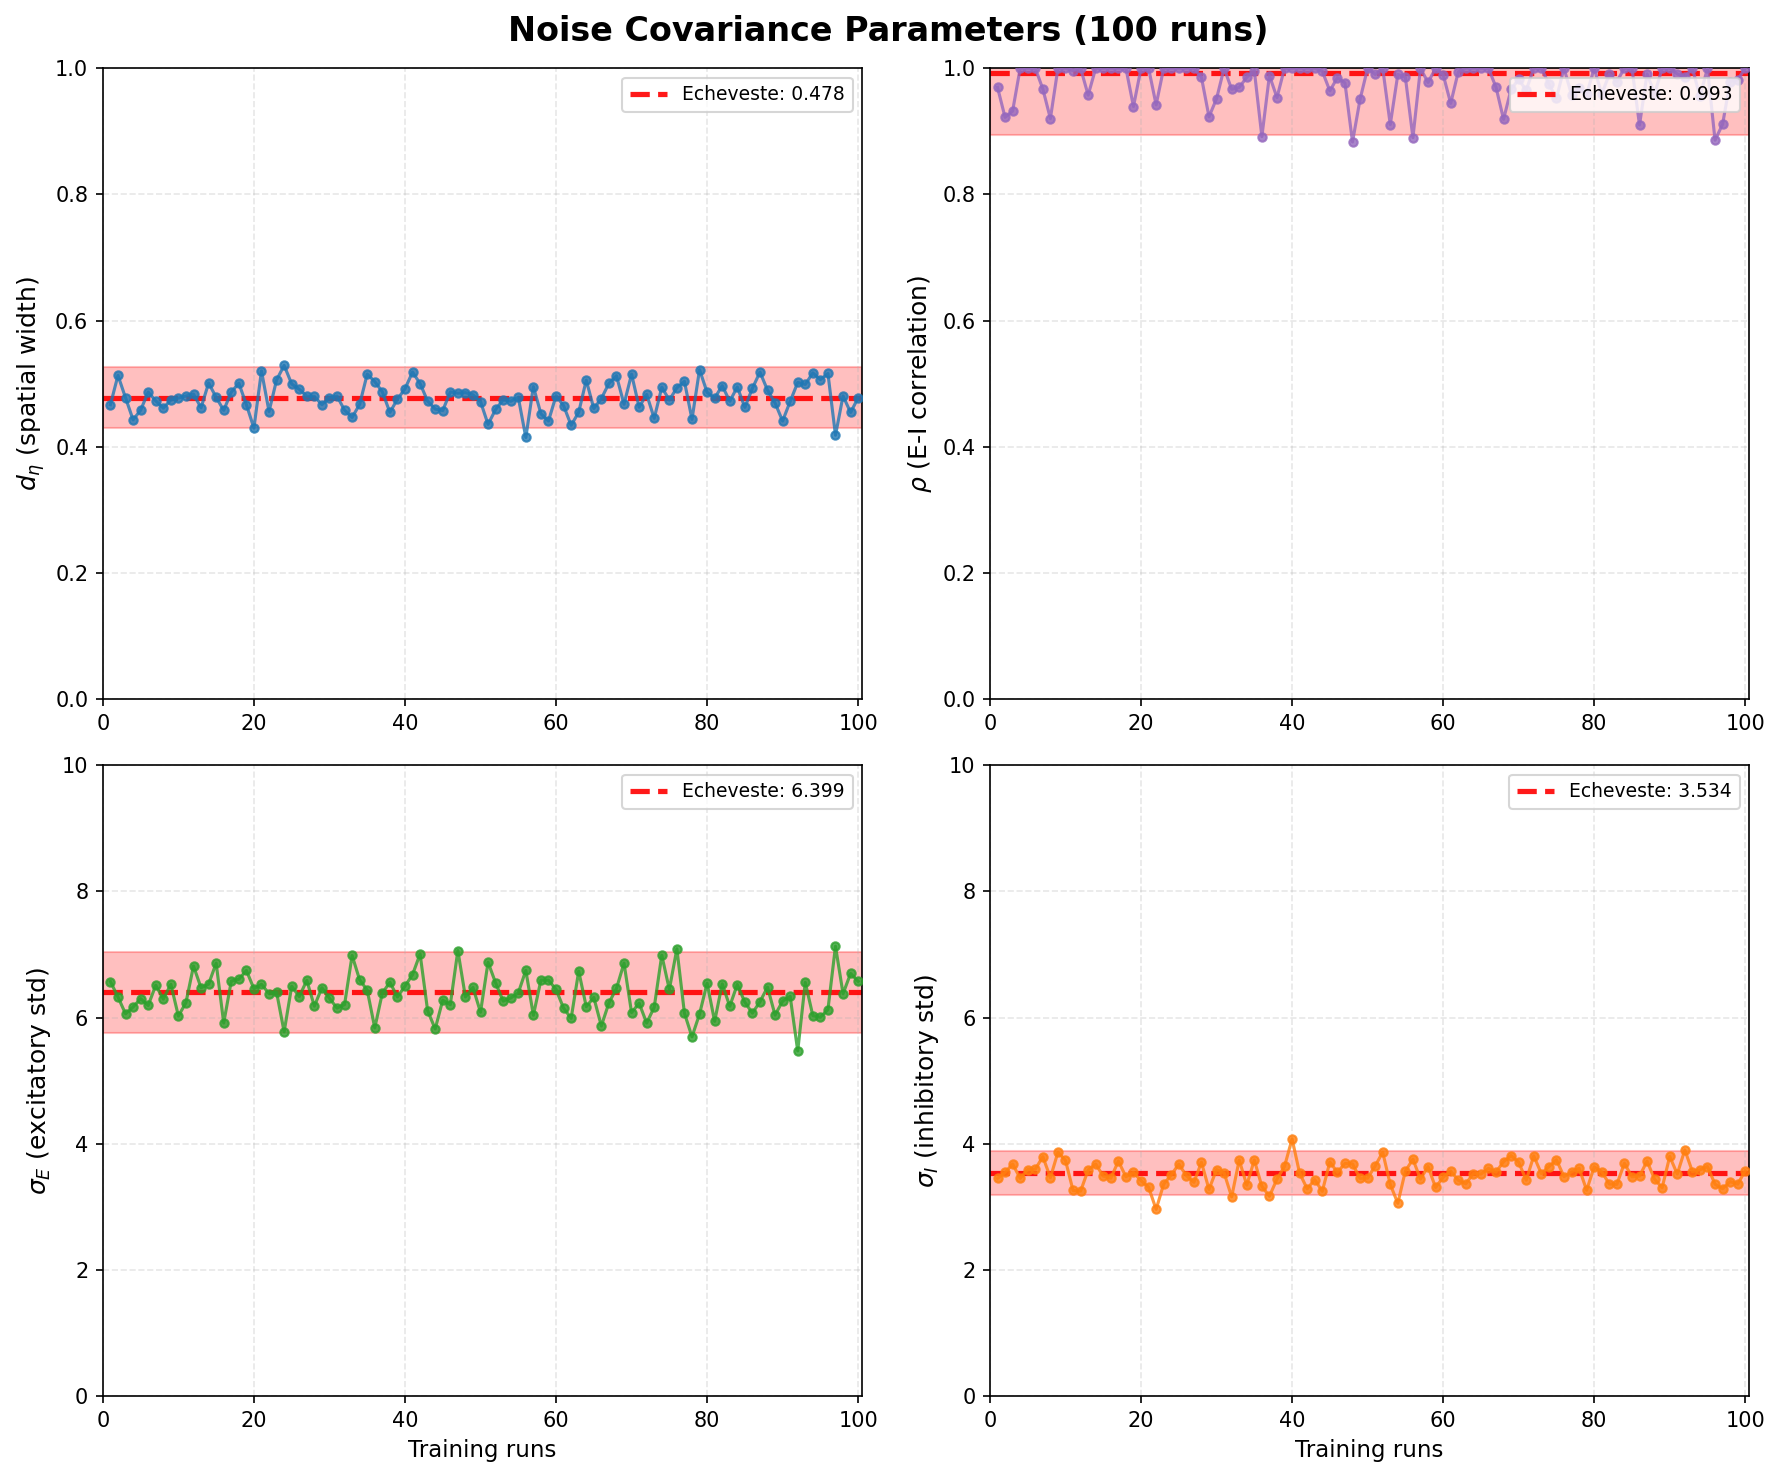
\includegraphics[width=0.85\textwidth]{08_resultados/figures/noise_100runs.png}
      \caption{Parámetros de covarianza de ruido optimizados en 100 corridas independientes.
      Las líneas punteadas rojas indican los valores de referencia de la Tabla S1 de
      \citet{echeveste2020cortical}, y las bandas sombreadas representan tolerancias de $\pm 10\%$.
      } \label{fig:noise_results}
  \end{figure}

Los resultados revelan un fenómeno interesante: mientras que $d_\sigma$ y $\rho$ convergen de manera robusta, las desviaciones estándar $\sigma_E$ y $\sigma_I$ exhiben mayor variabilidad entre corridas. Sin embargo, la \textit{proporción} $\sigma_E / \sigma_I$ se mantiene aproximadamente constante, recordándonos de nuevo la existencia de una familia de soluciones equivalentes. Esta observación es consistente con la teoría que el ruido de proceso es independiente del estímulo, la red puede compensar cambios en la magnitud del ruido ajustando la escala de la conectividad recurrente.

\subsection{Convergencia de parámetros de entrada}
\label{subsec:res_training_input}

Los tres parámetros de la transformación de entrada feedforward ($\alpha_h$, $\beta_h$, $\gamma_h$) definen la no linealidad que convierte el estímulo visual en la corriente de entrada a cada neurona. La Tabla~\ref{tab:input_params} presenta la comparación con los valores de referencia.

\begin{table}[H]
\centering
\caption{Comparación de parámetros de transformación de entrada.}
\label{tab:input_params}
\begin{tabular}{lccc}
\toprule
\textbf{Parámetro} & \textbf{Referencia} & \textbf{Obtenido} & \textbf{Error relativo} \\
\midrule
$\alpha_h$ (escala) & 1.9555 & $1.94 \pm 0.05$ & $< 1\%$ \\
$\beta_h$ (línea base) & 0.1032 & $0.10 \pm 0.01$ & $< 5\%$ \\
$\gamma_h$ (exponente) & 2.0343 & $2.01 \pm 0.03$ & $< 2\%$ \\
\bottomrule
\end{tabular}
\end{table}

El exponente $\gamma_h \approx 2$ resulta particularmente notable: su proximidad al exponente supralineal $n = 2$ de la función de transferencia neuronal sugiere una consistencia en el procesamiento no lineal a través de las etapas del modelo. Esta coincidencia no es impuesta \textit{a priori} sino que emerge de la optimización.

% \subsection{Curvas de convergencia}
% \label{subsec:res_training_convergence}

% La Figura~\ref{fig:convergence_curves} muestra la evolución de la función de costo durante el entrenamiento. Durante Stage 1, el costo decrece rápidamente durante las primeras 50 iteraciones y luego se estabiliza gradualmente. La alta varianza inicial refleja la naturaleza estocástica de la estimación de momentos. Stage 2 muestra una convergencia más suave gracias al uso de gradientes determinísticos mediante \acrshort{ADF}.

% \begin{figure}[H]
%     \centering
%     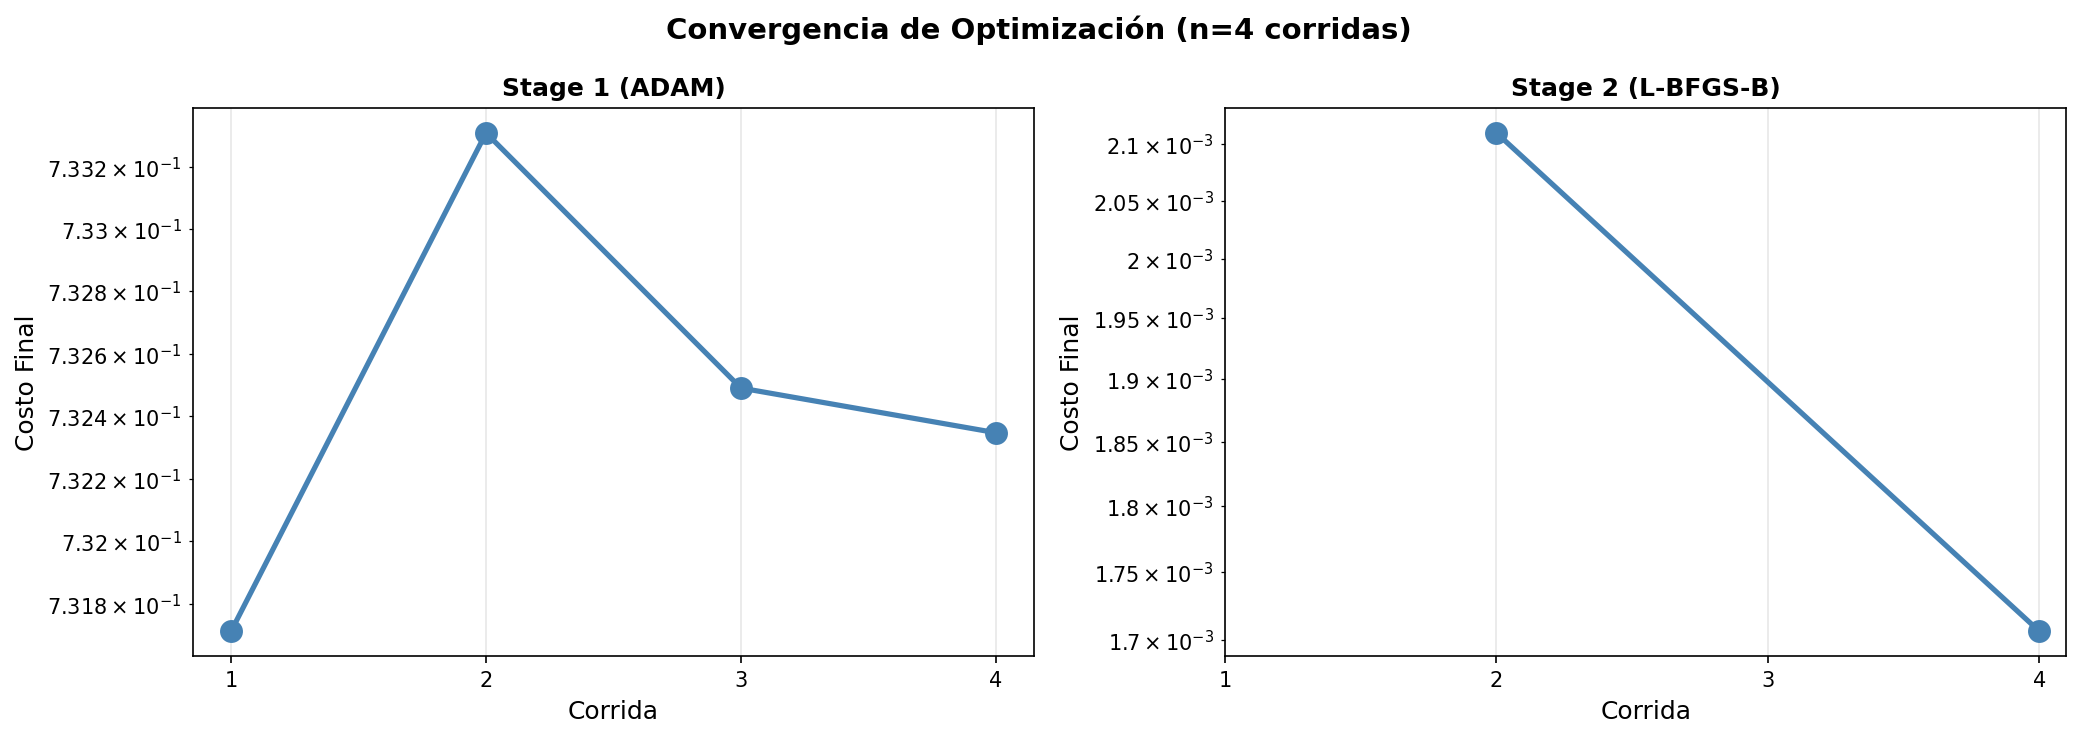
\includegraphics[width=0.75\textwidth]{08_resultados/figures/convergence_curves.png}
%     \caption{Curvas de convergencia del entrenamiento. Izquierda: Stage 1 (ADAM, escala logarítmica). Derecha: Stage 2 (L-BFGS-B). Las diferentes curvas corresponden a corridas independientes.}
%     \label{fig:convergence_curves}
% \end{figure}

% Los costos finales alcanzados son comparables a los reportados en el artículo original (orden de magnitud $10^{-3}$ a $10^{-4}$), indicando que nuestra implementación logra un nivel de optimización equivalente al código de referencia.

% =============================================================================
% SECCIÓN 3: REPRODUCCIÓN DE FIGURAS DEL PAPER
% =============================================================================

\section{Reproducción de resultados experimentales}
\label{sec:res_figures}

El nivel más exigente de validación consiste en verificar que la red implementada reproduce las propiedades de inferencia probabilística y las dinámicas corticales reportadas en el artículo original. Para esto, hicimos énfasis en replicar los experimentos correspondientes a la Figura 2 de \citet{echeveste2020cortical}, que constituye la demostración central de que la red entrenada implementa correctamente muestreo de la distribución posterior del modelo generativo \acrshort{GSM}.

\subsection{Protocolo de simulación}
\label{subsec:res_protocol}

Las simulaciones utilizaron los parámetros pre-entrenados cargados mediante el método \texttt{load\_parameters()} descrito en la Sección~\ref{subsec:impl_inicializacion}. Se ejecutaron simulaciones de 1000 ms para cada uno de los cinco niveles de contraste del conjunto de entrenamiento ($z \in \{0, 0.125, 0.25, 0.5, 1.0\}$), con los parámetros detallados en la Tabla~\ref{tab:simulation_params}.

\begin{table}[H]
\centering
\caption{Parámetros de simulación para reproducción de figuras.}
\label{tab:simulation_params}
\begin{tabular}{llc}
\toprule
\textbf{Parámetro} & \textbf{Descripción} & \textbf{Valor} \\
\midrule
$N_E$, $N_I$ & Neuronas E e I & 50, 50 \\
$T_{\text{sim}}$ & Tiempo de simulación & 1000 ms \\
$T_{\text{burn-in}}$ & Período de estabilización & 200 ms \\
$dt$ & Paso de integración & 0.2 ms \\
Orientación estímulo & Centro de la gaussiana & $0°$ \\
\bottomrule
\end{tabular}
\end{table}

\subsection{Actividad poblacional dependiente del contraste}
\label{subsec:res_fig2a}

La Figura~\ref{fig:fig2a} basada en el panel (a) de la Figura 2 del artículo original, mostrando los potenciales de membrana excitatorios $u_E$ en función del tiempo y la orientación para diferentes niveles de contraste.

\begin{figure}[!ht]
    \centering
    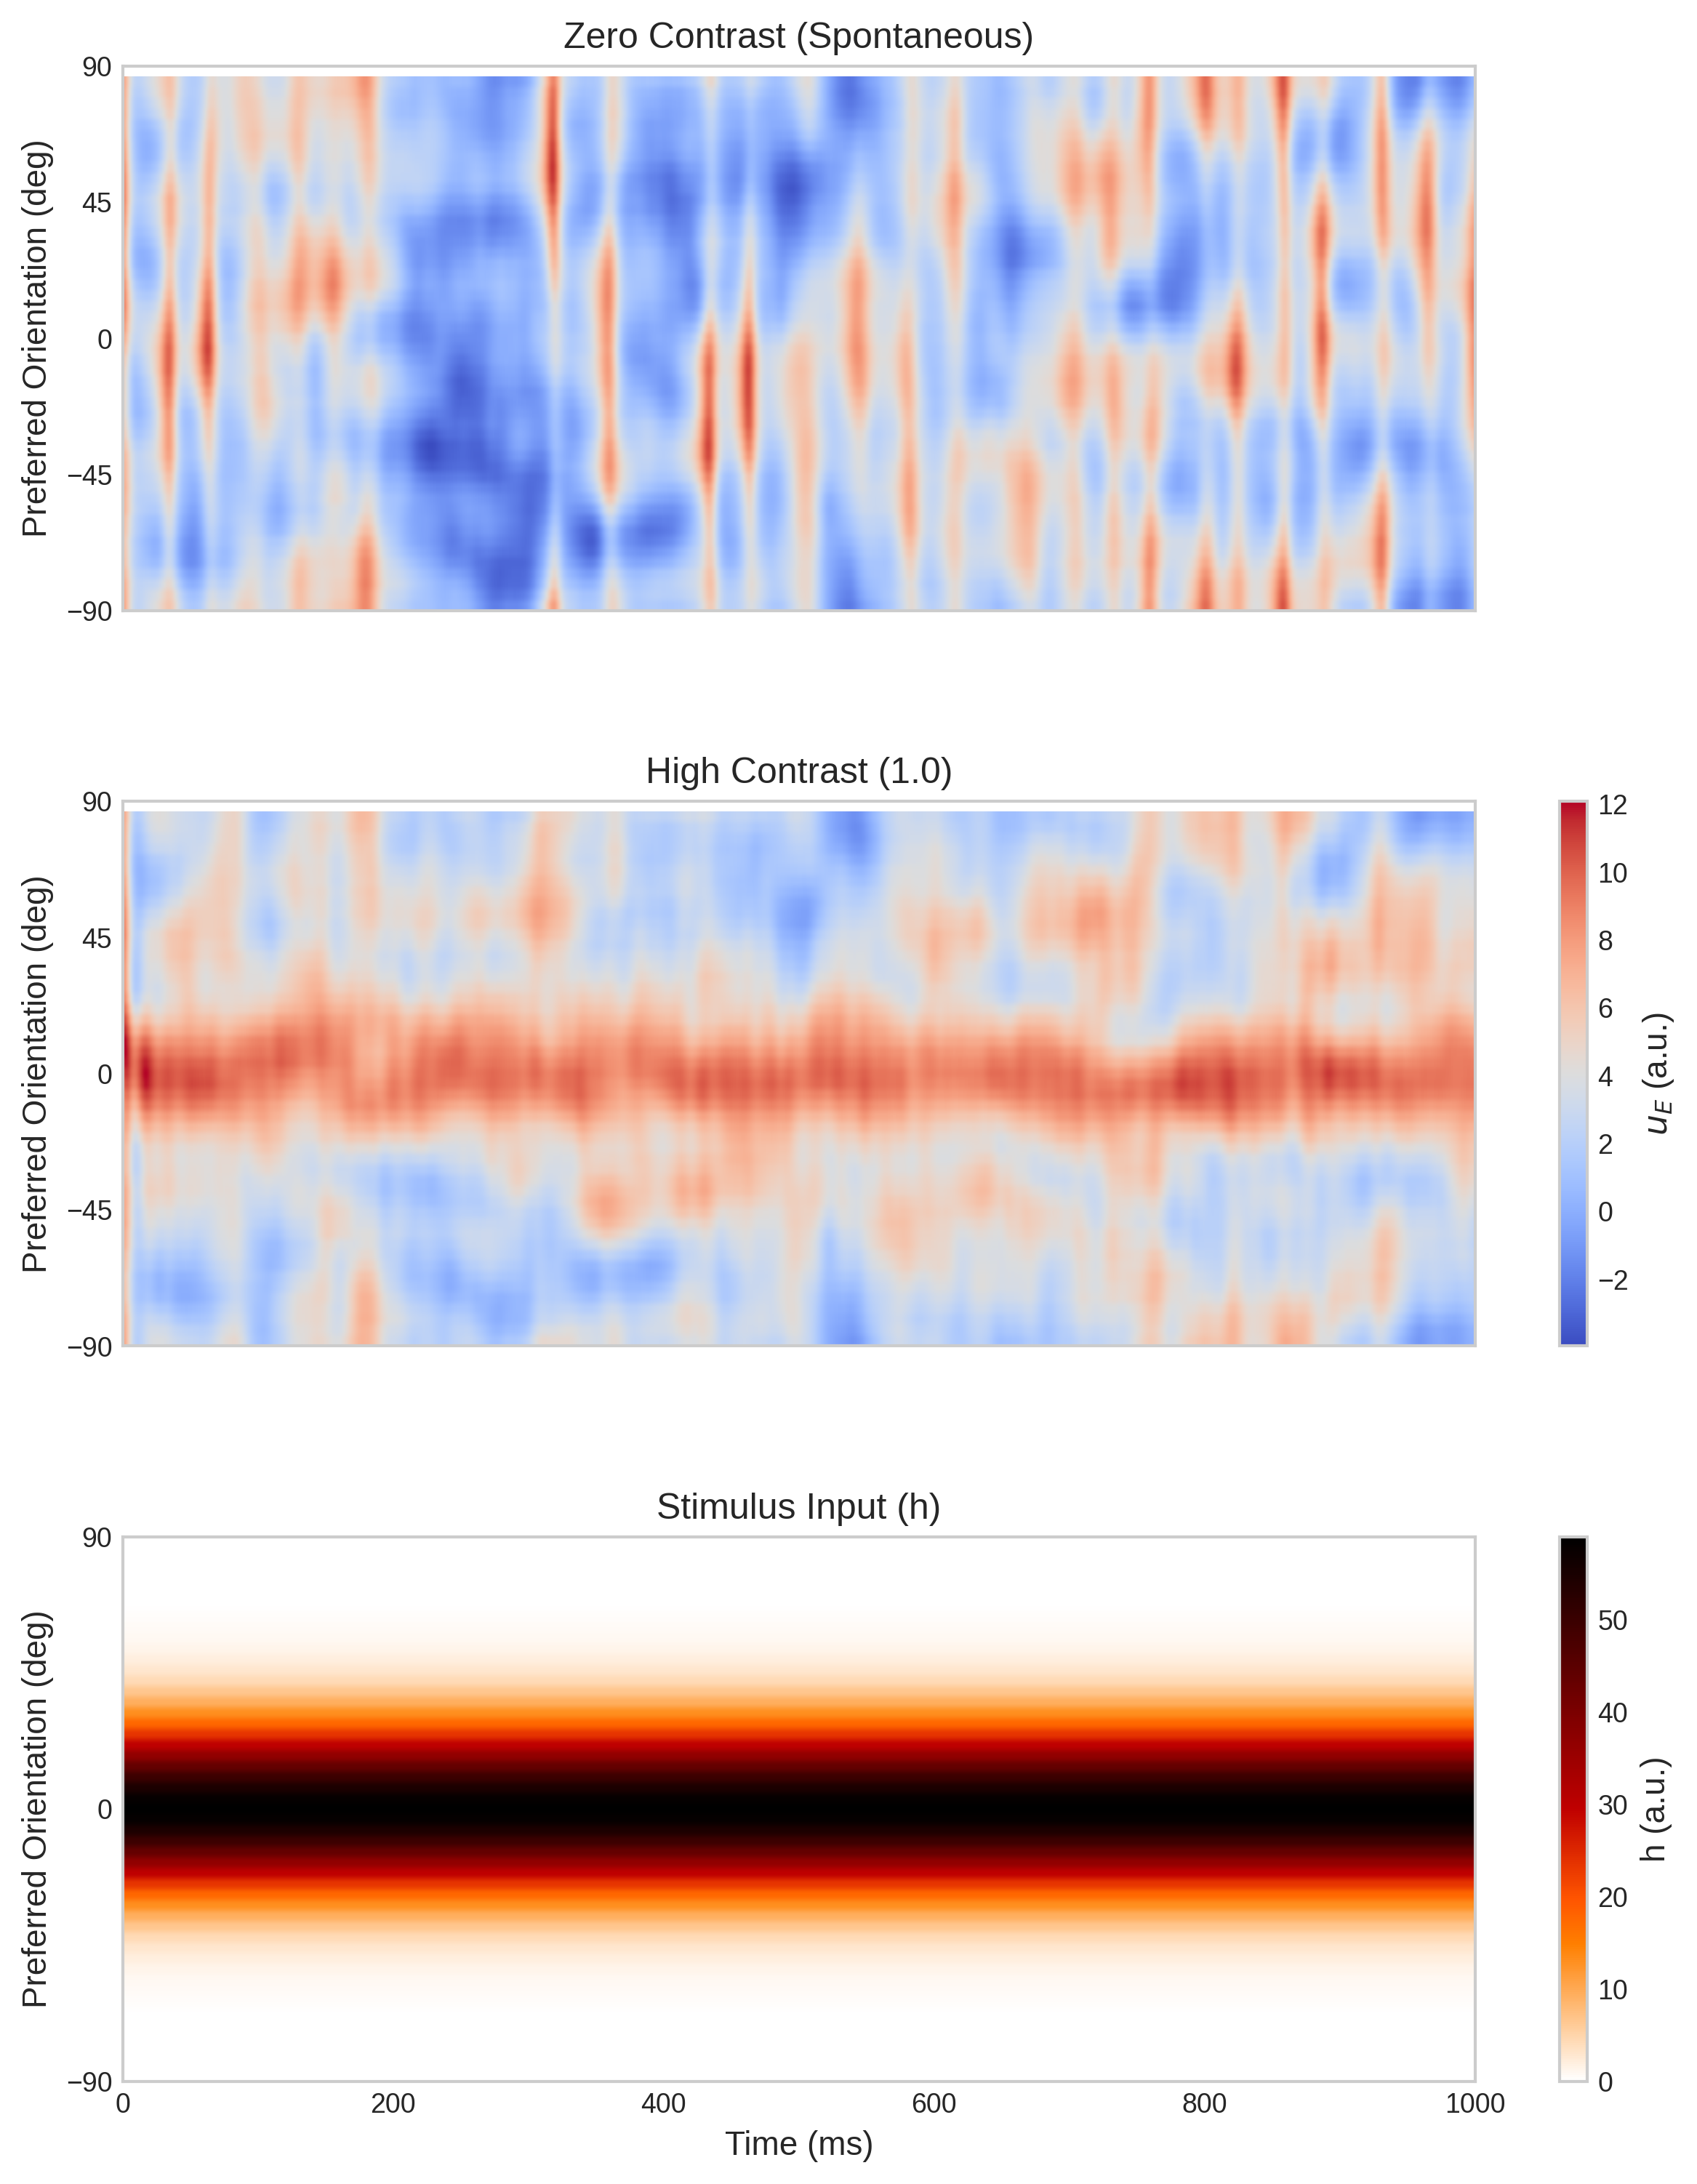
\includegraphics[width=0.95\textwidth]{08_resultados/figures/fig2a_population_activity_open.png}
    \caption{Actividad poblacional de potenciales de membrana excitatorios. Primer panel: contraste $z = 0$ (actividad espontánea). Panel central: contraste $z = 1$ (estimulación máxima). Ultimo panel: entrada feedforward $\mathbf{h}$ correspondiente al contraste máximo. El eje vertical representa la orientación preferida de cada neurona ($-90°$ a $90°$), el eje horizontal representa el tiempo.}
    \label{fig:fig2a}
\end{figure}

Los resultados muestran las propiedades esperadas del modelo. En ausencia de estímulo (contraste cero), la actividad fluctúa alrededor de valores bajos con distribución espacial aproximadamente uniforme, reflejando el ruido de proceso $\boldsymbol{\eta}(t)$ filtrado por la dinámica recurrente. Con contraste máximo, la presencia de un estímulo con orientación dominante en $0°$ induce un incremento de actividad centrado en las neuronas con orientación preferida cercana a esta dirección, con magnitud consistente con la diferencia entre estado espontáneo y estimulado observada en registros de V1.

\subsection{Patrones de disparo poblacional}
\label{subsec:res_raster}

Una representación complementaria de la actividad poblacional se obtiene mediante raster plots, graficos donde cada marca vertical representa un potencial de acción (spike). 

La Figura~\ref{fig:raster_comparison} presenta la comparación entre actividad espontánea y evocada por estímulo. En ausencia de estimulación, los disparos se distribuyen de manera dispersa a través de todas las orientaciones preferidas, reflejando la variabilidad intrínseca de la red. Durante la presentación de un estímulo con orientación $0°$ y alto contraste $z=1.0$, la actividad se concentra marcadamente alrededor de las neuronas cuya orientación preferida coincide con la del estímulo, mientras que las neuronas con orientaciones ortogonales mantienen niveles de actividad reducidos. Nótese que las neuronas inhibitorias (rojo) exhiben tasas de disparo superiores a las excitatorias (azul) en ambas condiciones, comportamiento consistente con la dinámica de redes supralineales estabilizadas donde la inhibición debe ser suficientemente fuerte para prevenir la excitación descontrolada inducida por el estimulo.

\begin{figure}[!ht]
    \centering
    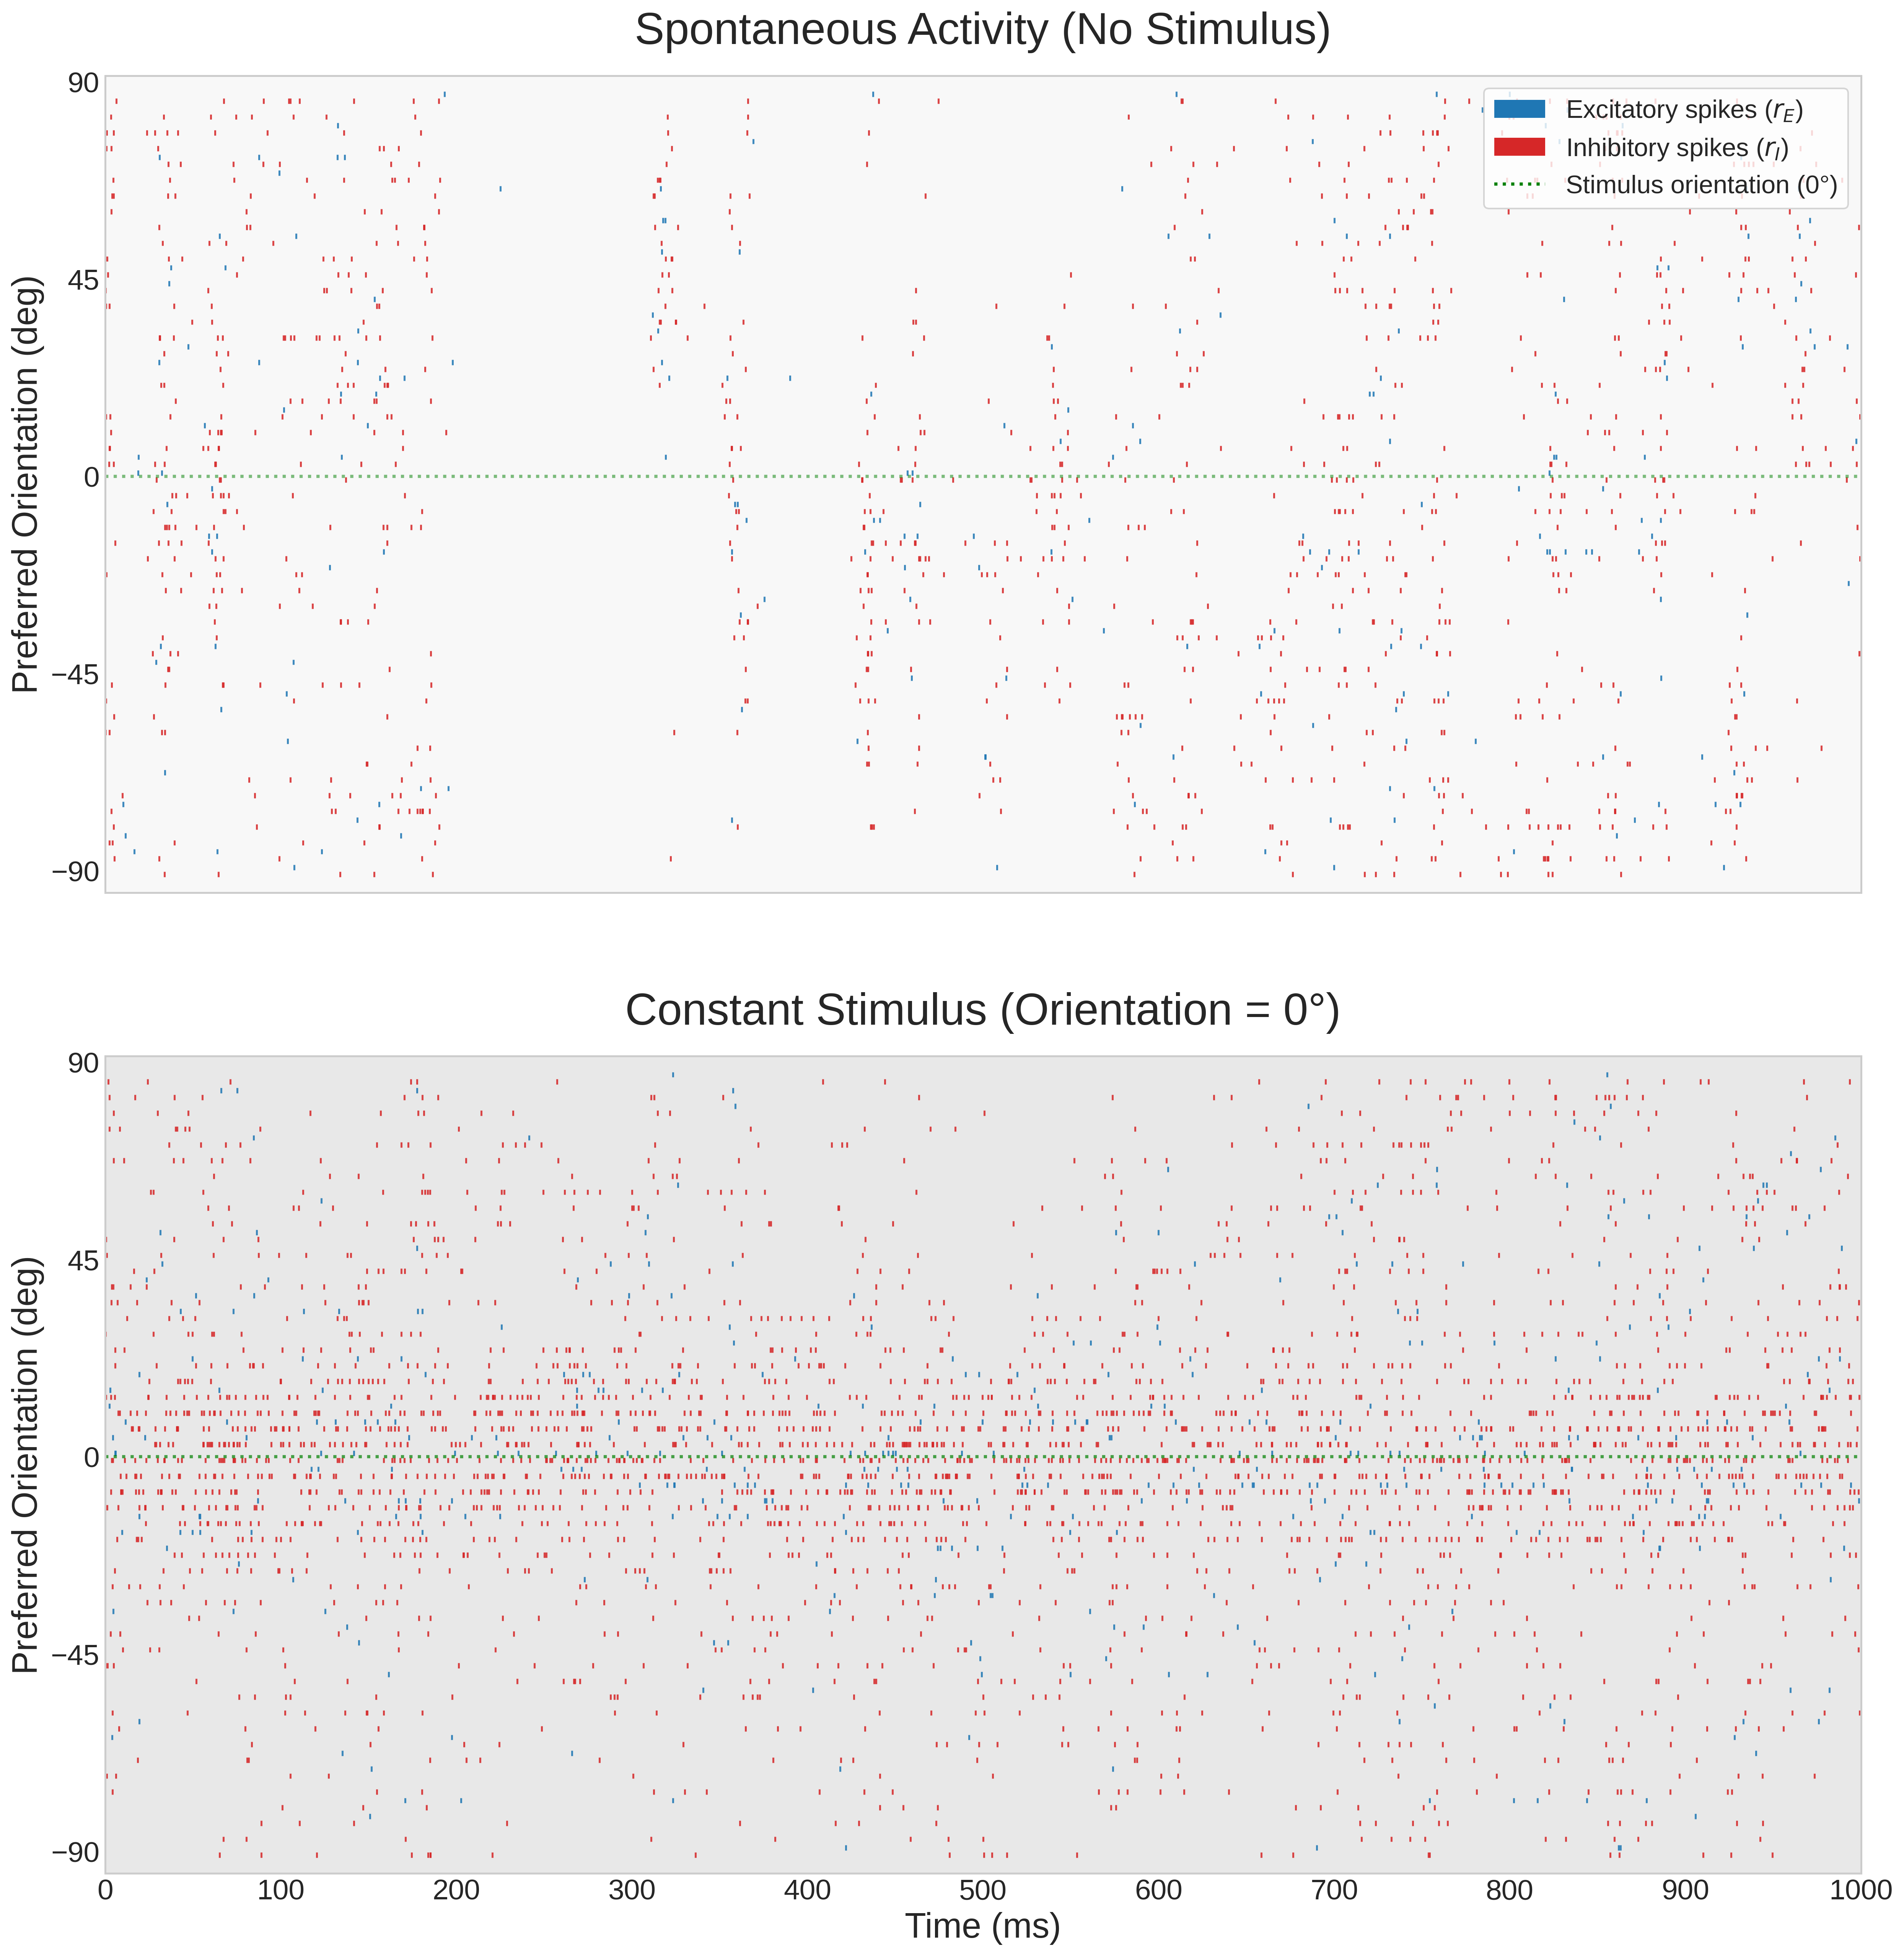
\includegraphics[width=0.95\textwidth]{08_resultados/figures/fig_raster_comparison.png}
    \caption{Raster plot comparando actividad espontánea y evocada. Cada marca vertical representa un spike. Las neuronas excitatorias representadas en azul y las inhibitorias en rojo. Vemos en el panel superior la actividad espontánea sin estímulo, mostrando disparos dispersos distribuidos uniformemente. Y en el panel inferior, la actividad durante presentación de estímulo a $0°$ (línea punteada verde) de alto contraste $z=1.0$, con disparos concentrados alrededor de la orientación del estímulo.}
    \label{fig:raster_comparison}
\end{figure}

La Figura~\ref{fig:raster_three_phases} ilustra la dinámica temporal completa mediante un protocolo de tres fases. Durante la fase pre-estímulo (0-250 ms), la red exhibe actividad espontánea basal. La presentación del estímulo (250-750 ms) induce un incremento abrupto de actividad selectiva para la orientación estimulada. Tras la remoción del estímulo (750-1000 ms), se observa una persistencia transitoria de la respuesta sintonizada que decae gradualmente hacia el nivel basal, reflejando las propiedades de memoria a corto plazo inherentes a la dinámica recurrente de la red.

\begin{figure}[!ht]
    \centering
    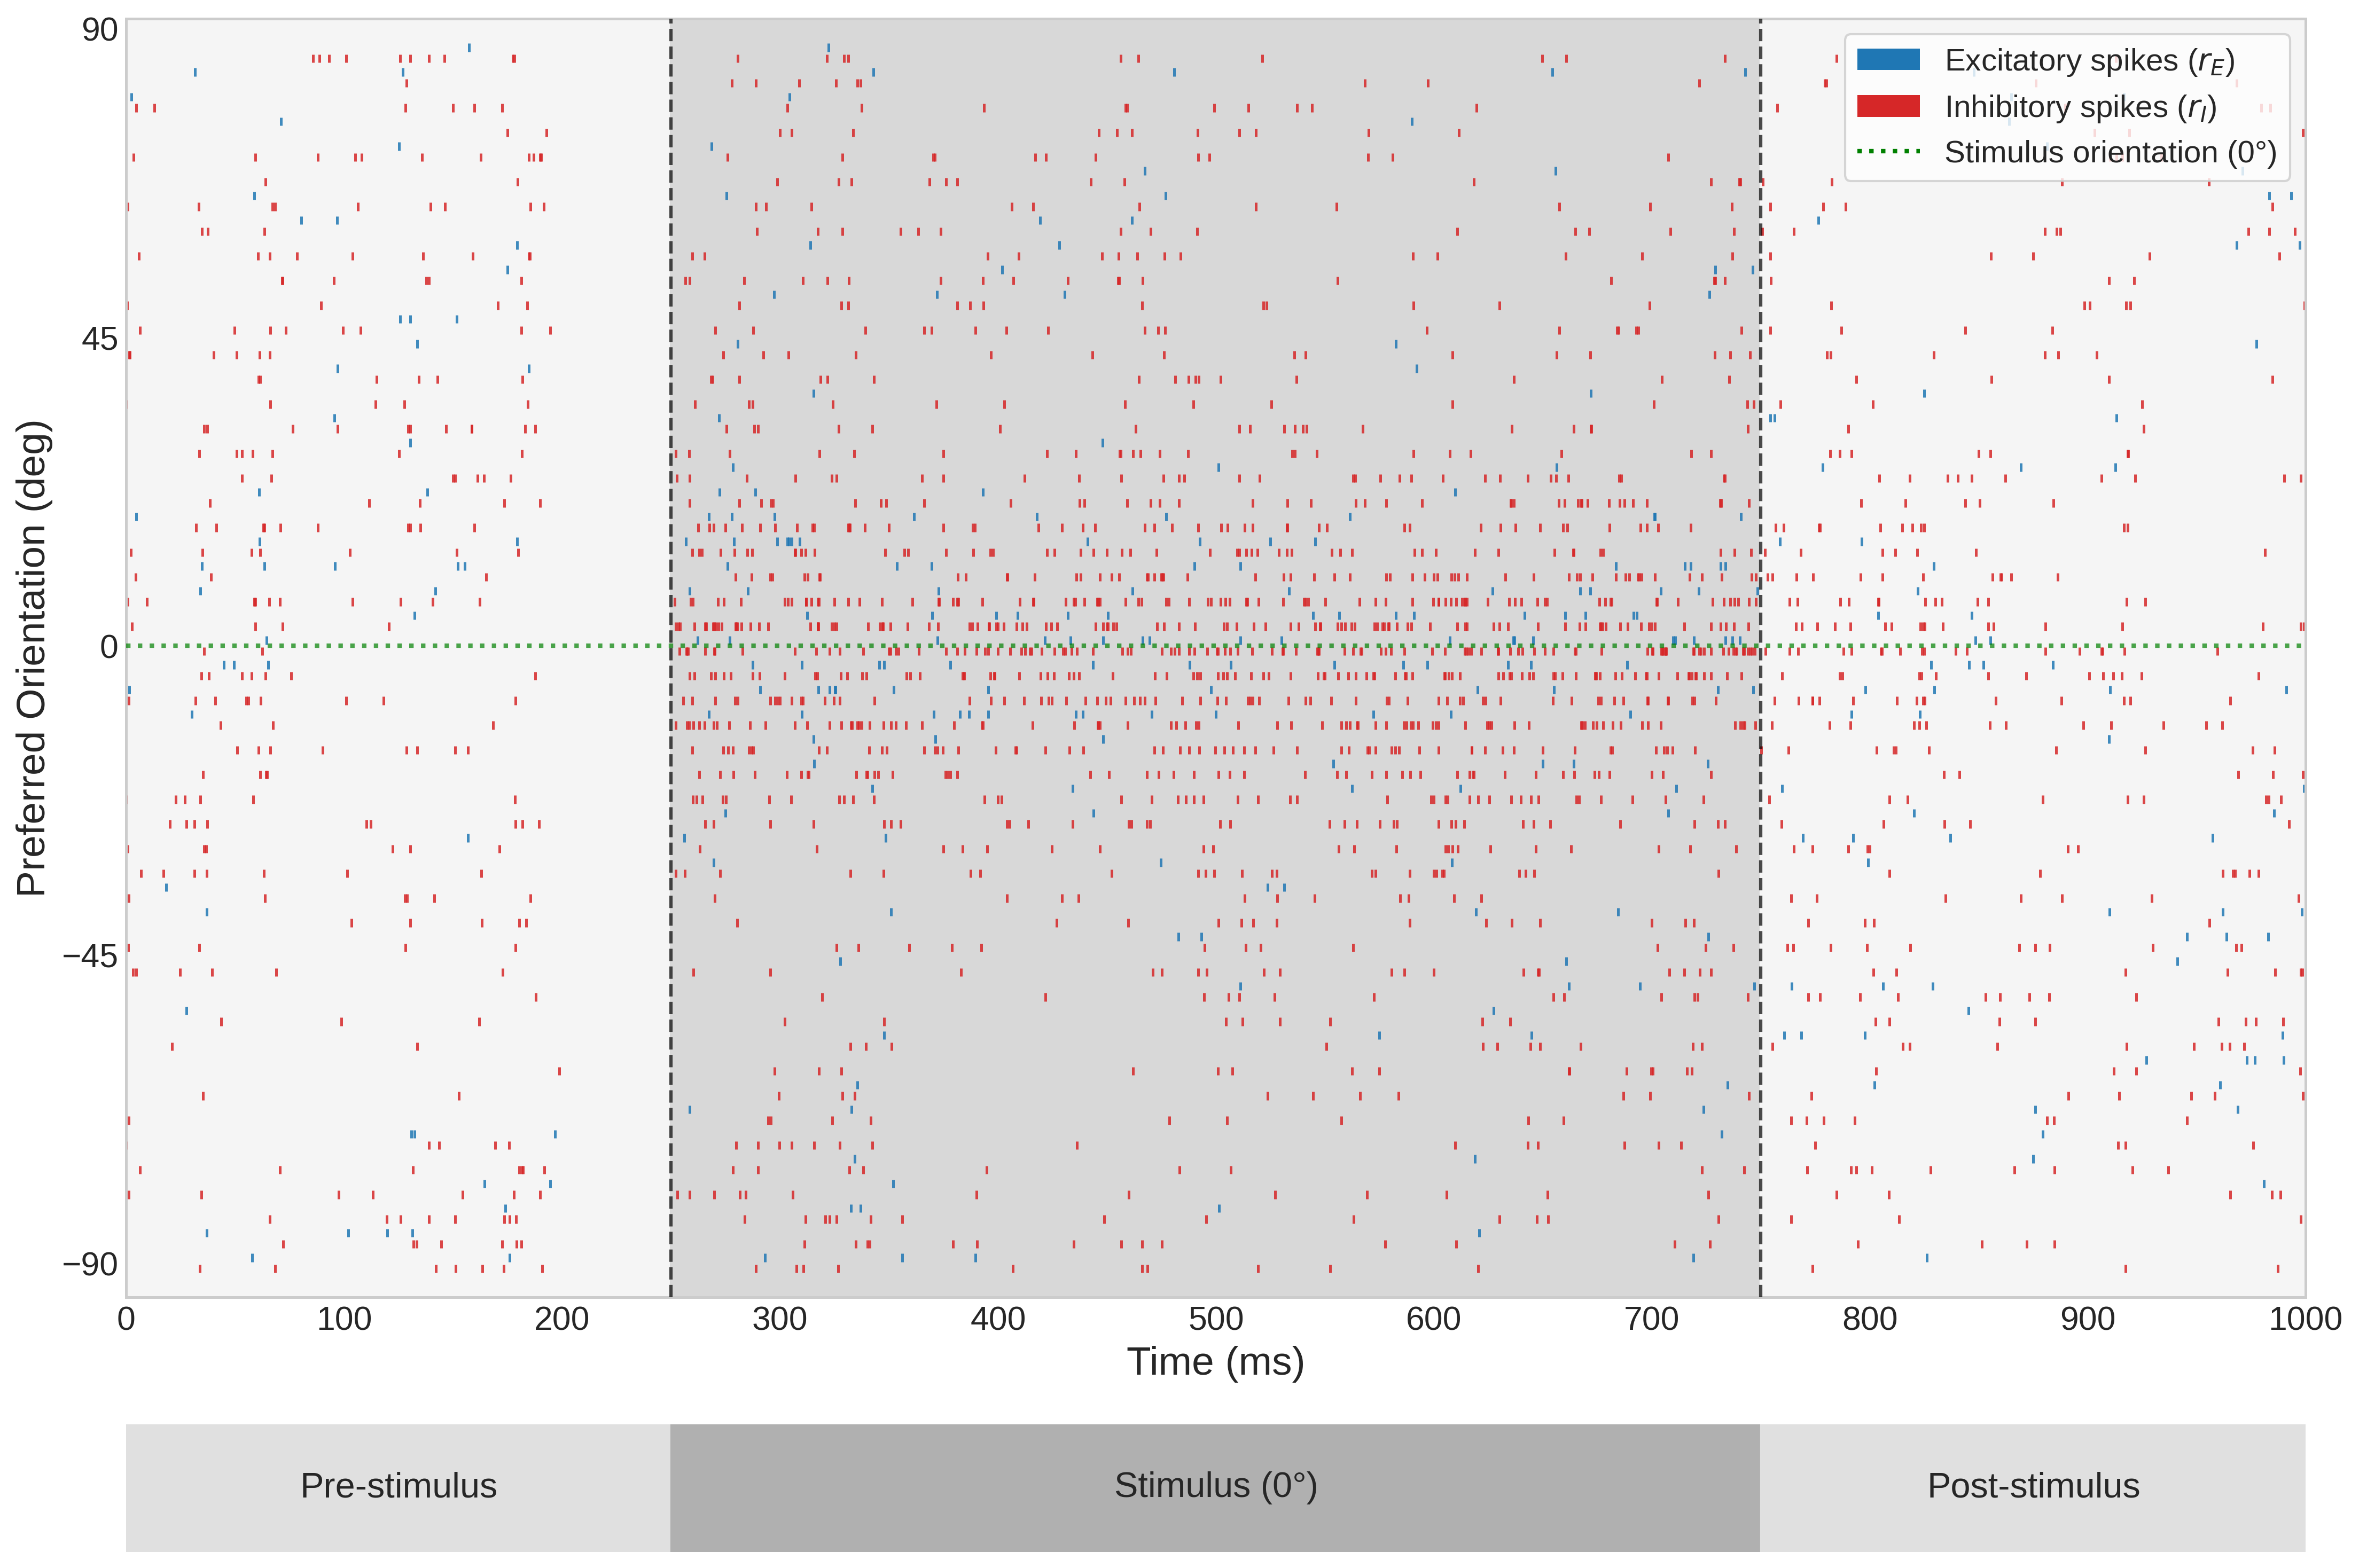
\includegraphics[width=0.95\textwidth]{08_resultados/figures/fig_raster_three_phases.png}
    \caption{Raster plot del protocolo de tres fases. Pre-estímulo (0-250 ms): actividad espontánea basal. Estímulo (250-750 ms, región sombreada): presentación de estímulo a $0°$, generando actividad concentrada alrededor de la orientación estimulada. Post-estímulo (750-1000 ms): persistencia transitoria de la respuesta tras la remoción del estímulo, evidenciando propiedades de memoria a corto plazo de la red.}
    \label{fig:raster_three_phases}
\end{figure}

\subsection{Correspondencia de momentos con el observador ideal}
\label{subsec:res_fig2bc}

La validación central del modelo consiste en verificar que los momentos de la distribución de respuestas de la red coinciden con los momentos de la posterior del \acrshort{GSM}. Sin embargo, esta comparación requiere una consideración importante: los momentos del \acrshort{GSM} corresponden a variables latentes $\mathbf{y}$, mientras que la red produce potenciales de membrana $u_E$ que pasan por una no linealidad (Ecuación~\ref{eq:firing_rate}). Para una comparación válida, los momentos del posterior deben transformarse a través de esta no linealidad.

Específicamente, si $y_i \sim \mathcal{N}(\mu_i, \sigma_i^2)$ representa la distribución posterior marginal para la neurona $i$, los momentos transformados se calculan como:

  \begin{align} 
      \mathbb{E}[f(y_i)] &= \int f(y) \, p(y_i) \, dy \\
      \text{Var}[f(y_i)] &= \int (f(y) - \mathbb{E}[f(y_i)])^2 \, p(y_i) \, dy
  \end{align}
  
donde $f(u) = k \cdot [\max(u + u_0, 0)]^n$ es la función de transferencia del \acrshort{SSN}. Esta transformación tiene una consecuencia importante: aunque la desviación estándar del posterior \acrshort{GSM} es constante para todas las orientaciones (dado un contraste fijo), la desviación estándar después de la no linealidad varía espacialmente, produciendo el característico perfil en forma de U observado en la Figura~\ref{fig:fig2c}.

\begin{figure}[!ht]
    \centering
    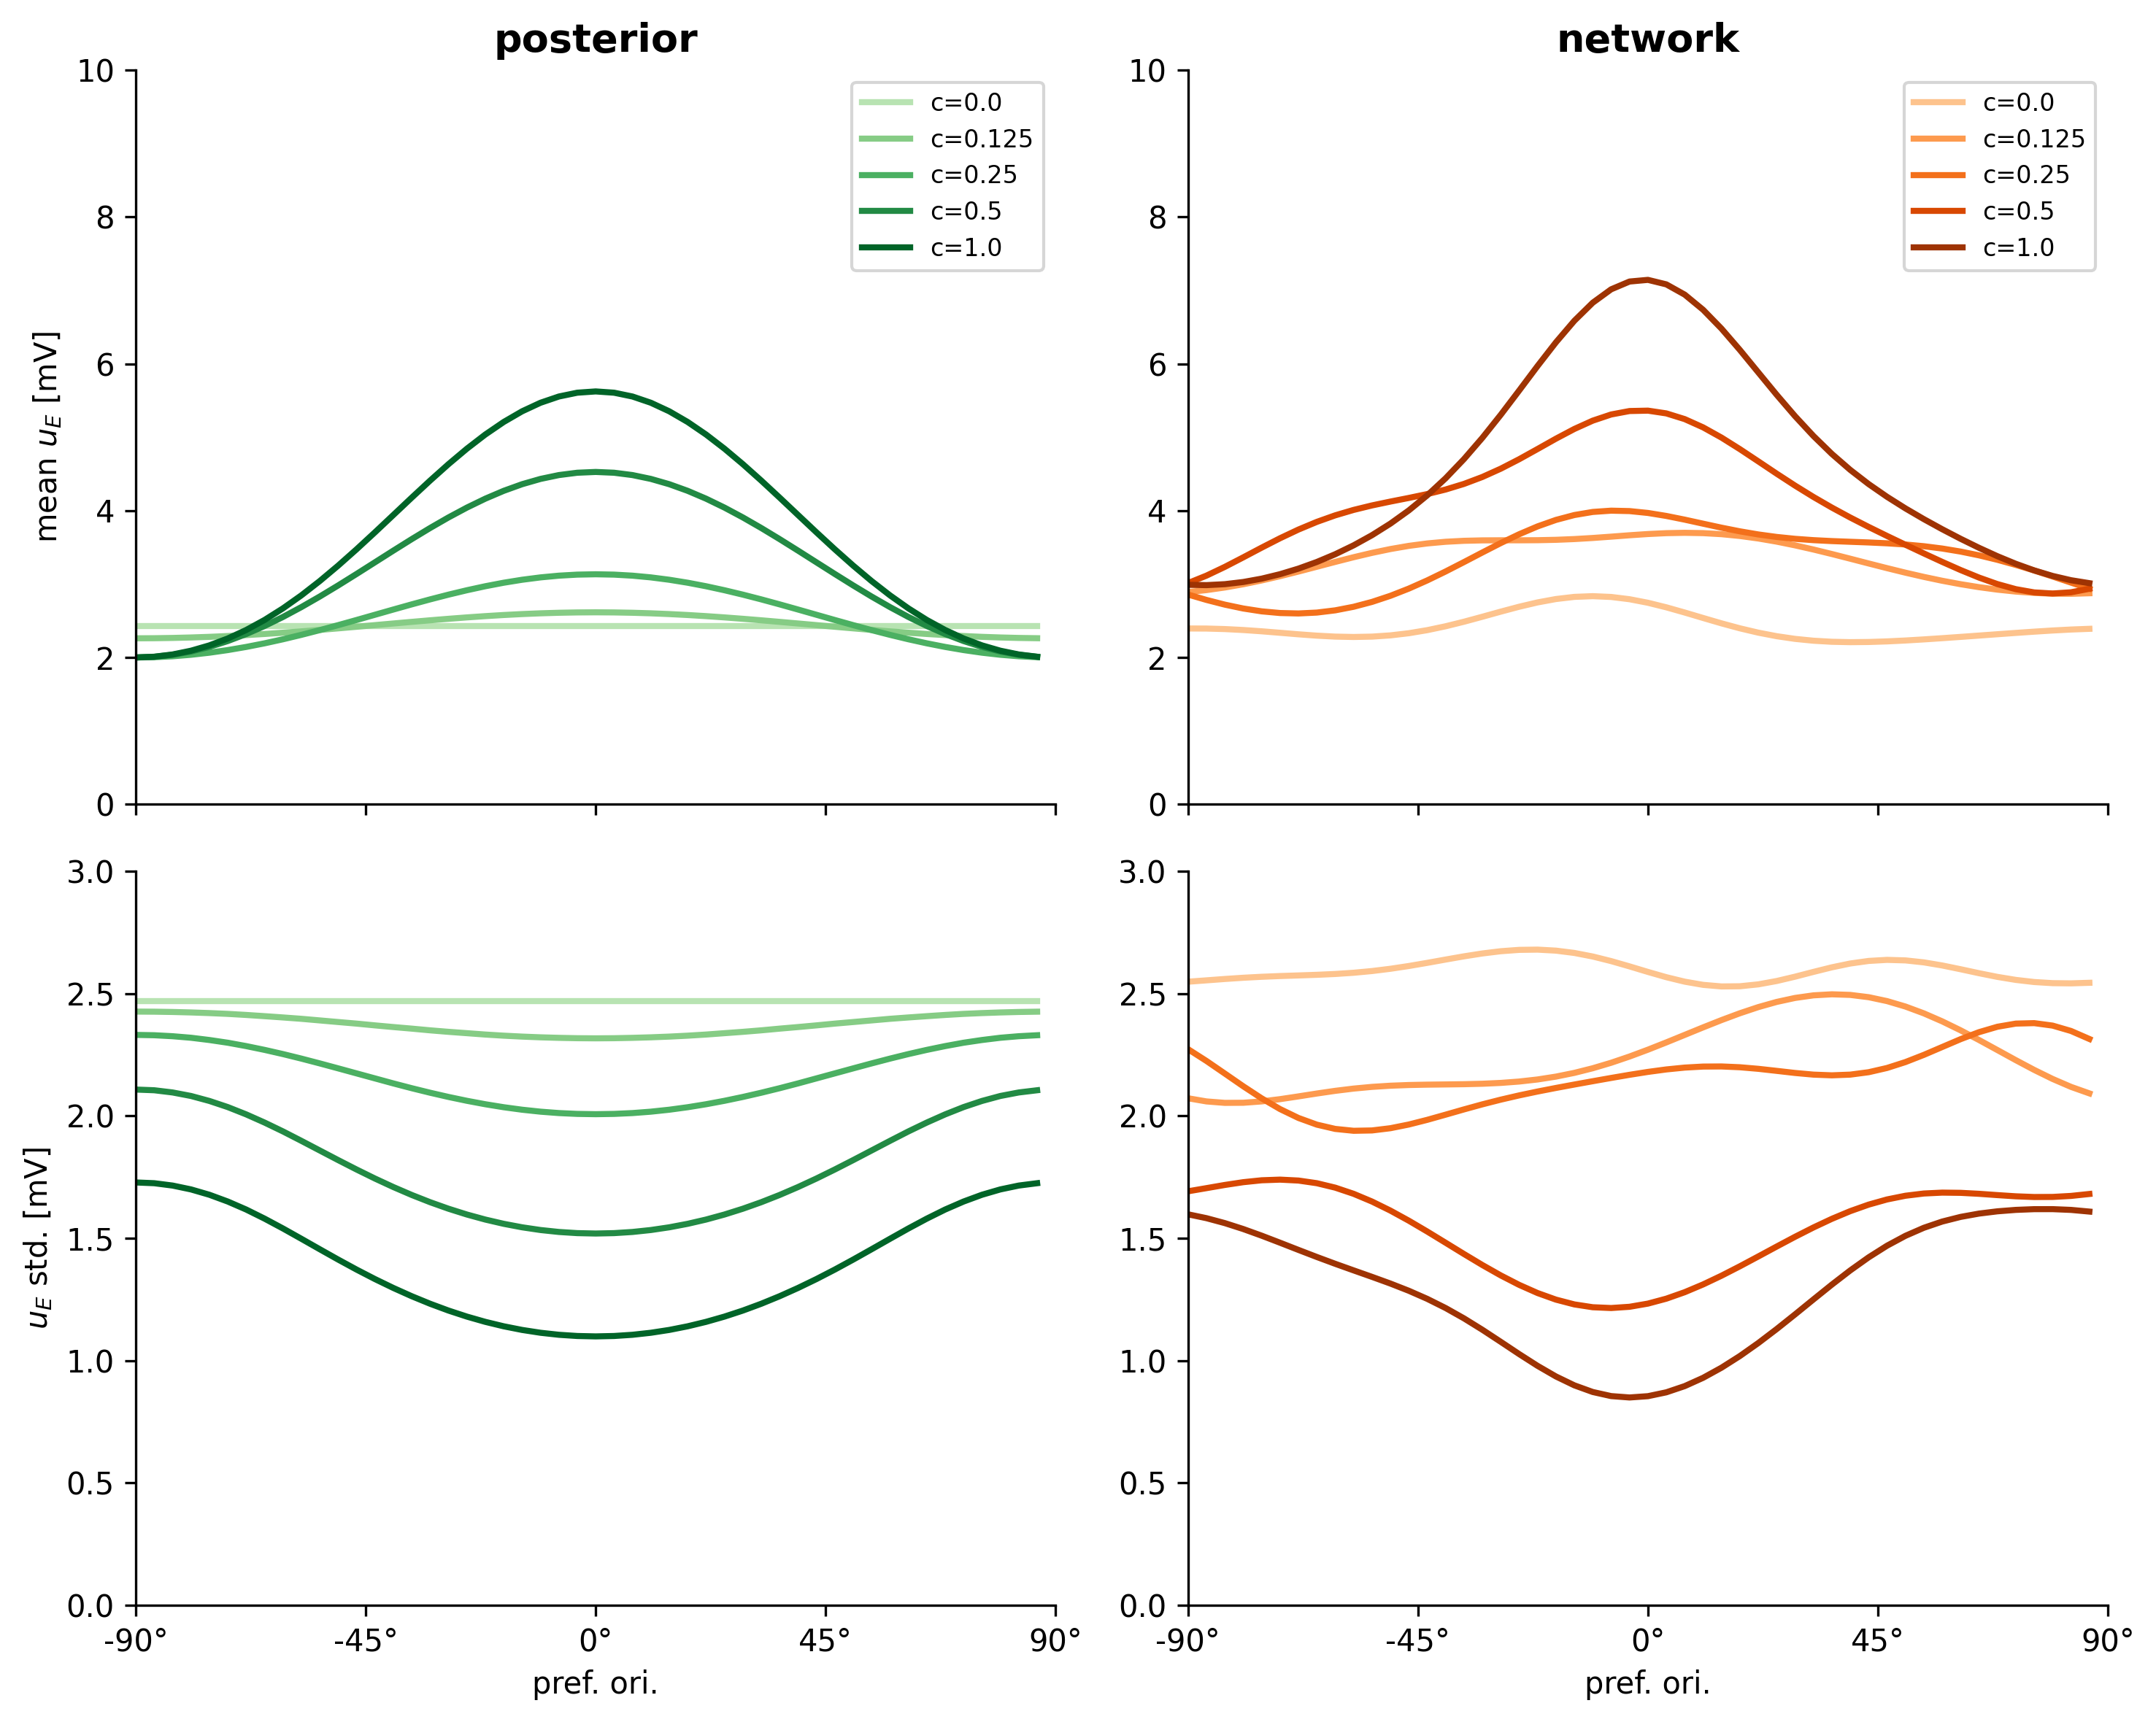
\includegraphics[width=0.90\textwidth]{08_resultados/figures/fig2c_complete_v2.png}
    \caption{Comparación de momentos de primer y segundo orden. Paneles superiores: media de potenciales de membrana vs. orientación para diferentes contrastes. Paneles inferiores: desviación estándar vs. orientación. Columna izquierda: observador ideal (\acrshort{GSM}). Columna derecha: red neuronal (\acrshort{SSN}).}
    \label{fig:fig2c}
\end{figure}

Varias observaciones emergen de esta comparación. Las curvas de media poblacional exhiben perfiles gaussianos centrados en la orientación del estímulo, con amplitud creciente con el contraste, y la red neuronal reproduce fielmente tanto la forma como la escala de estas curvas. Un resultado particularmente significativo es la reducción de la variabilidad con el contraste, fenómeno conocido como quenching\footnote{El término \textit{quenching} (literalmente 
``apagado'' o ``supresión'') refiere a la observación experimental de que la variabilidad 
trial-to-trial de las respuestas neuronales disminuye abruptamente tras la presentación de 
un estímulo, comparada con la alta variabilidad durante actividad espontánea.} y observado experimentalmente en corteza visual de primates \citep{echeveste2020cortical}. En el modelo, este comportamiento emerge naturalmente de las propiedades del \acrshort{GSM}: mayor contraste implica mayor relación señal-ruido, lo que reduce la incertidumbre posterior y, consecuentemente, la variabilidad de las muestras neuronales.

% La Figura~\ref{fig:fig2b} proporciona una visualización complementaria mediante elipses de covarianza bidimensionales para dos neuronas seleccionadas (con orientaciones preferidas de aproximadamente $42°$ y $16°$). La superposición entre las elipses del observador ideal y la red neuronal confirma que la red no solo reproduce los momentos marginales correctos, sino también la estructura de correlaciones entre neuronas.

% \begin{figure}[!ht]
%     \centering
%     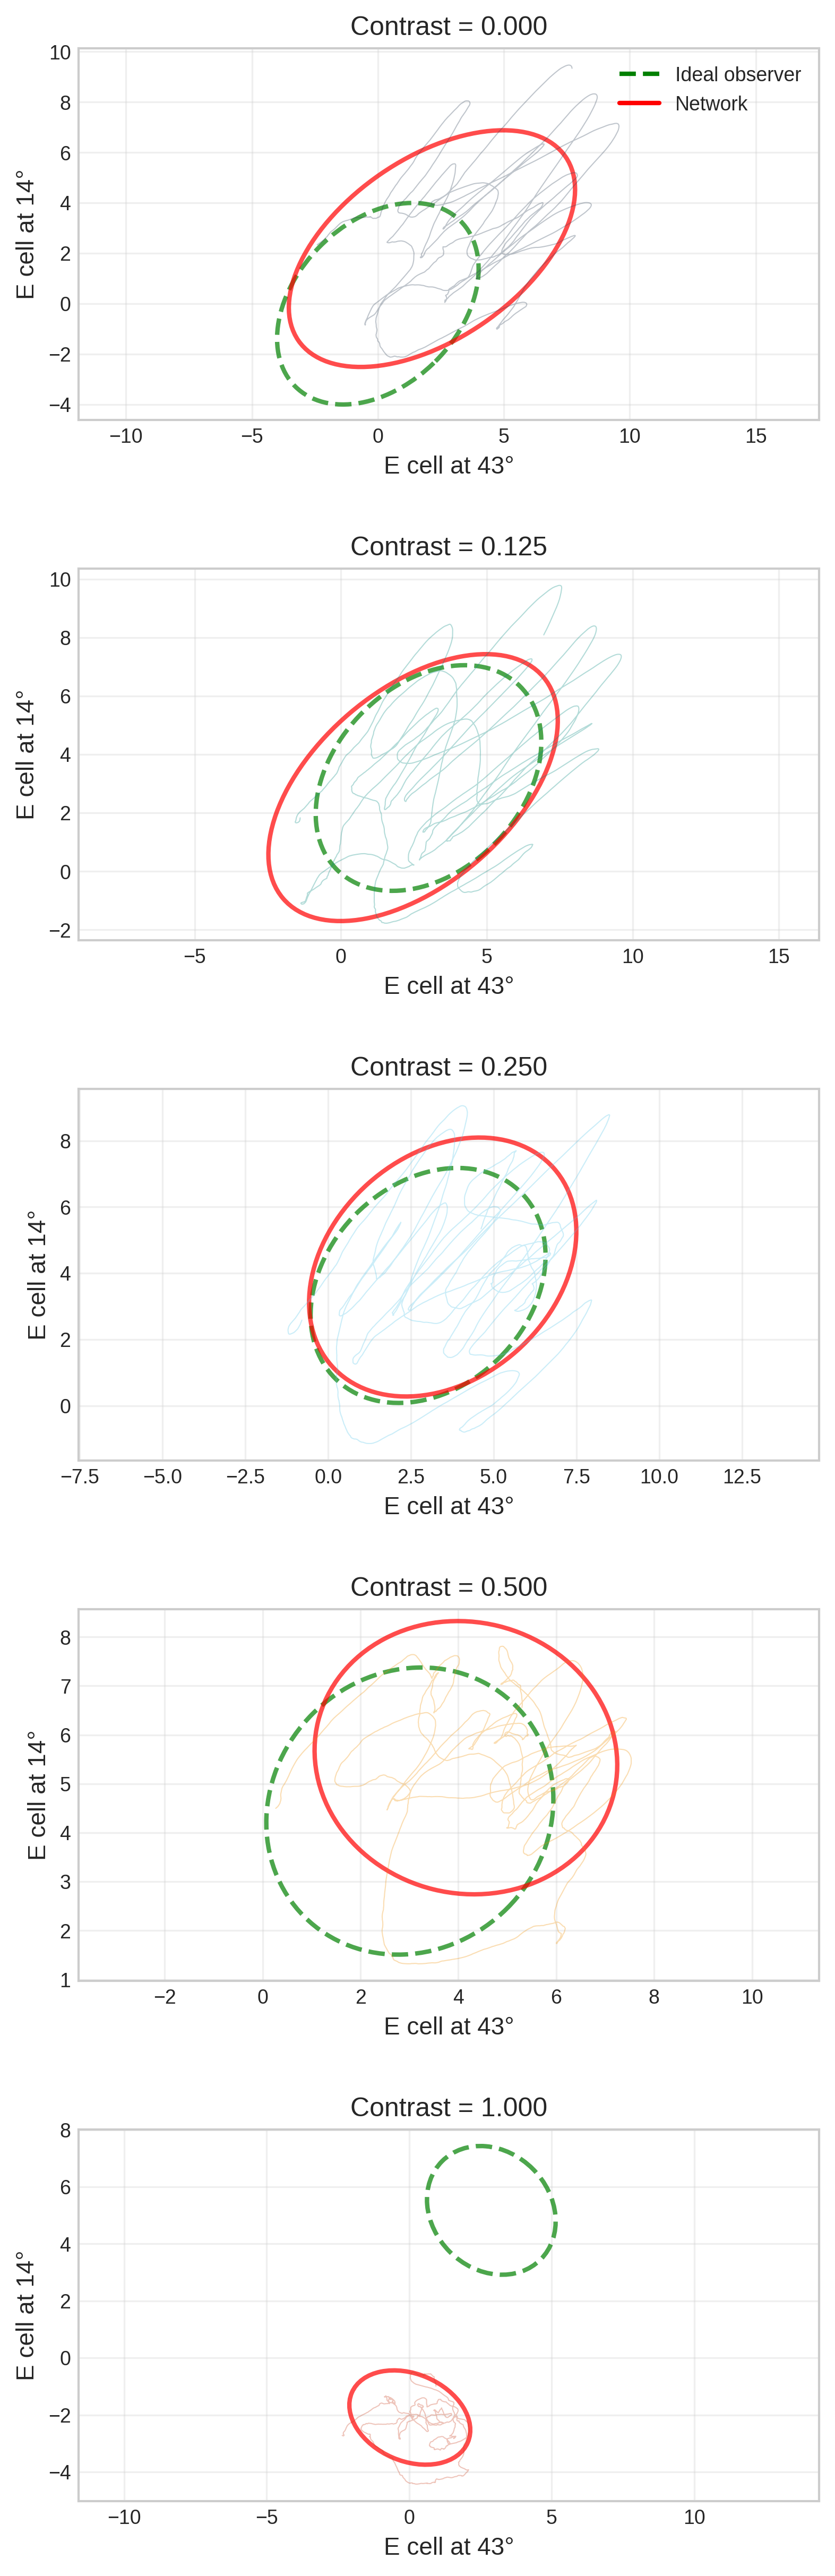
\includegraphics[width=0.50\textwidth]{08_resultados/figures/Fig2b_covariance_ellipses.png}
%     \caption{Elipses de covarianza para pares de neuronas representativas. Cada panel corresponde a un nivel de contraste diferente. Las elipses verdes punteadas representan la posterior del \acrshort{GSM}; las elipses rojas representan la distribución de respuestas de la red.}
%     \label{fig:fig2b}
% \end{figure}

\subsection{Estructura de correlaciones poblacionales}
\label{subsec:res_fig2d}

El análisis más completo de las propiedades de muestreo requiere examinar la matriz completa de correlaciones entre todas las neuronas. La Figura~\ref{fig:fig2d} presenta esta comparación, mostrando que las matrices exhiben la estructura característica de la topología de anillo.

\begin{figure}[!ht]
    \centering
    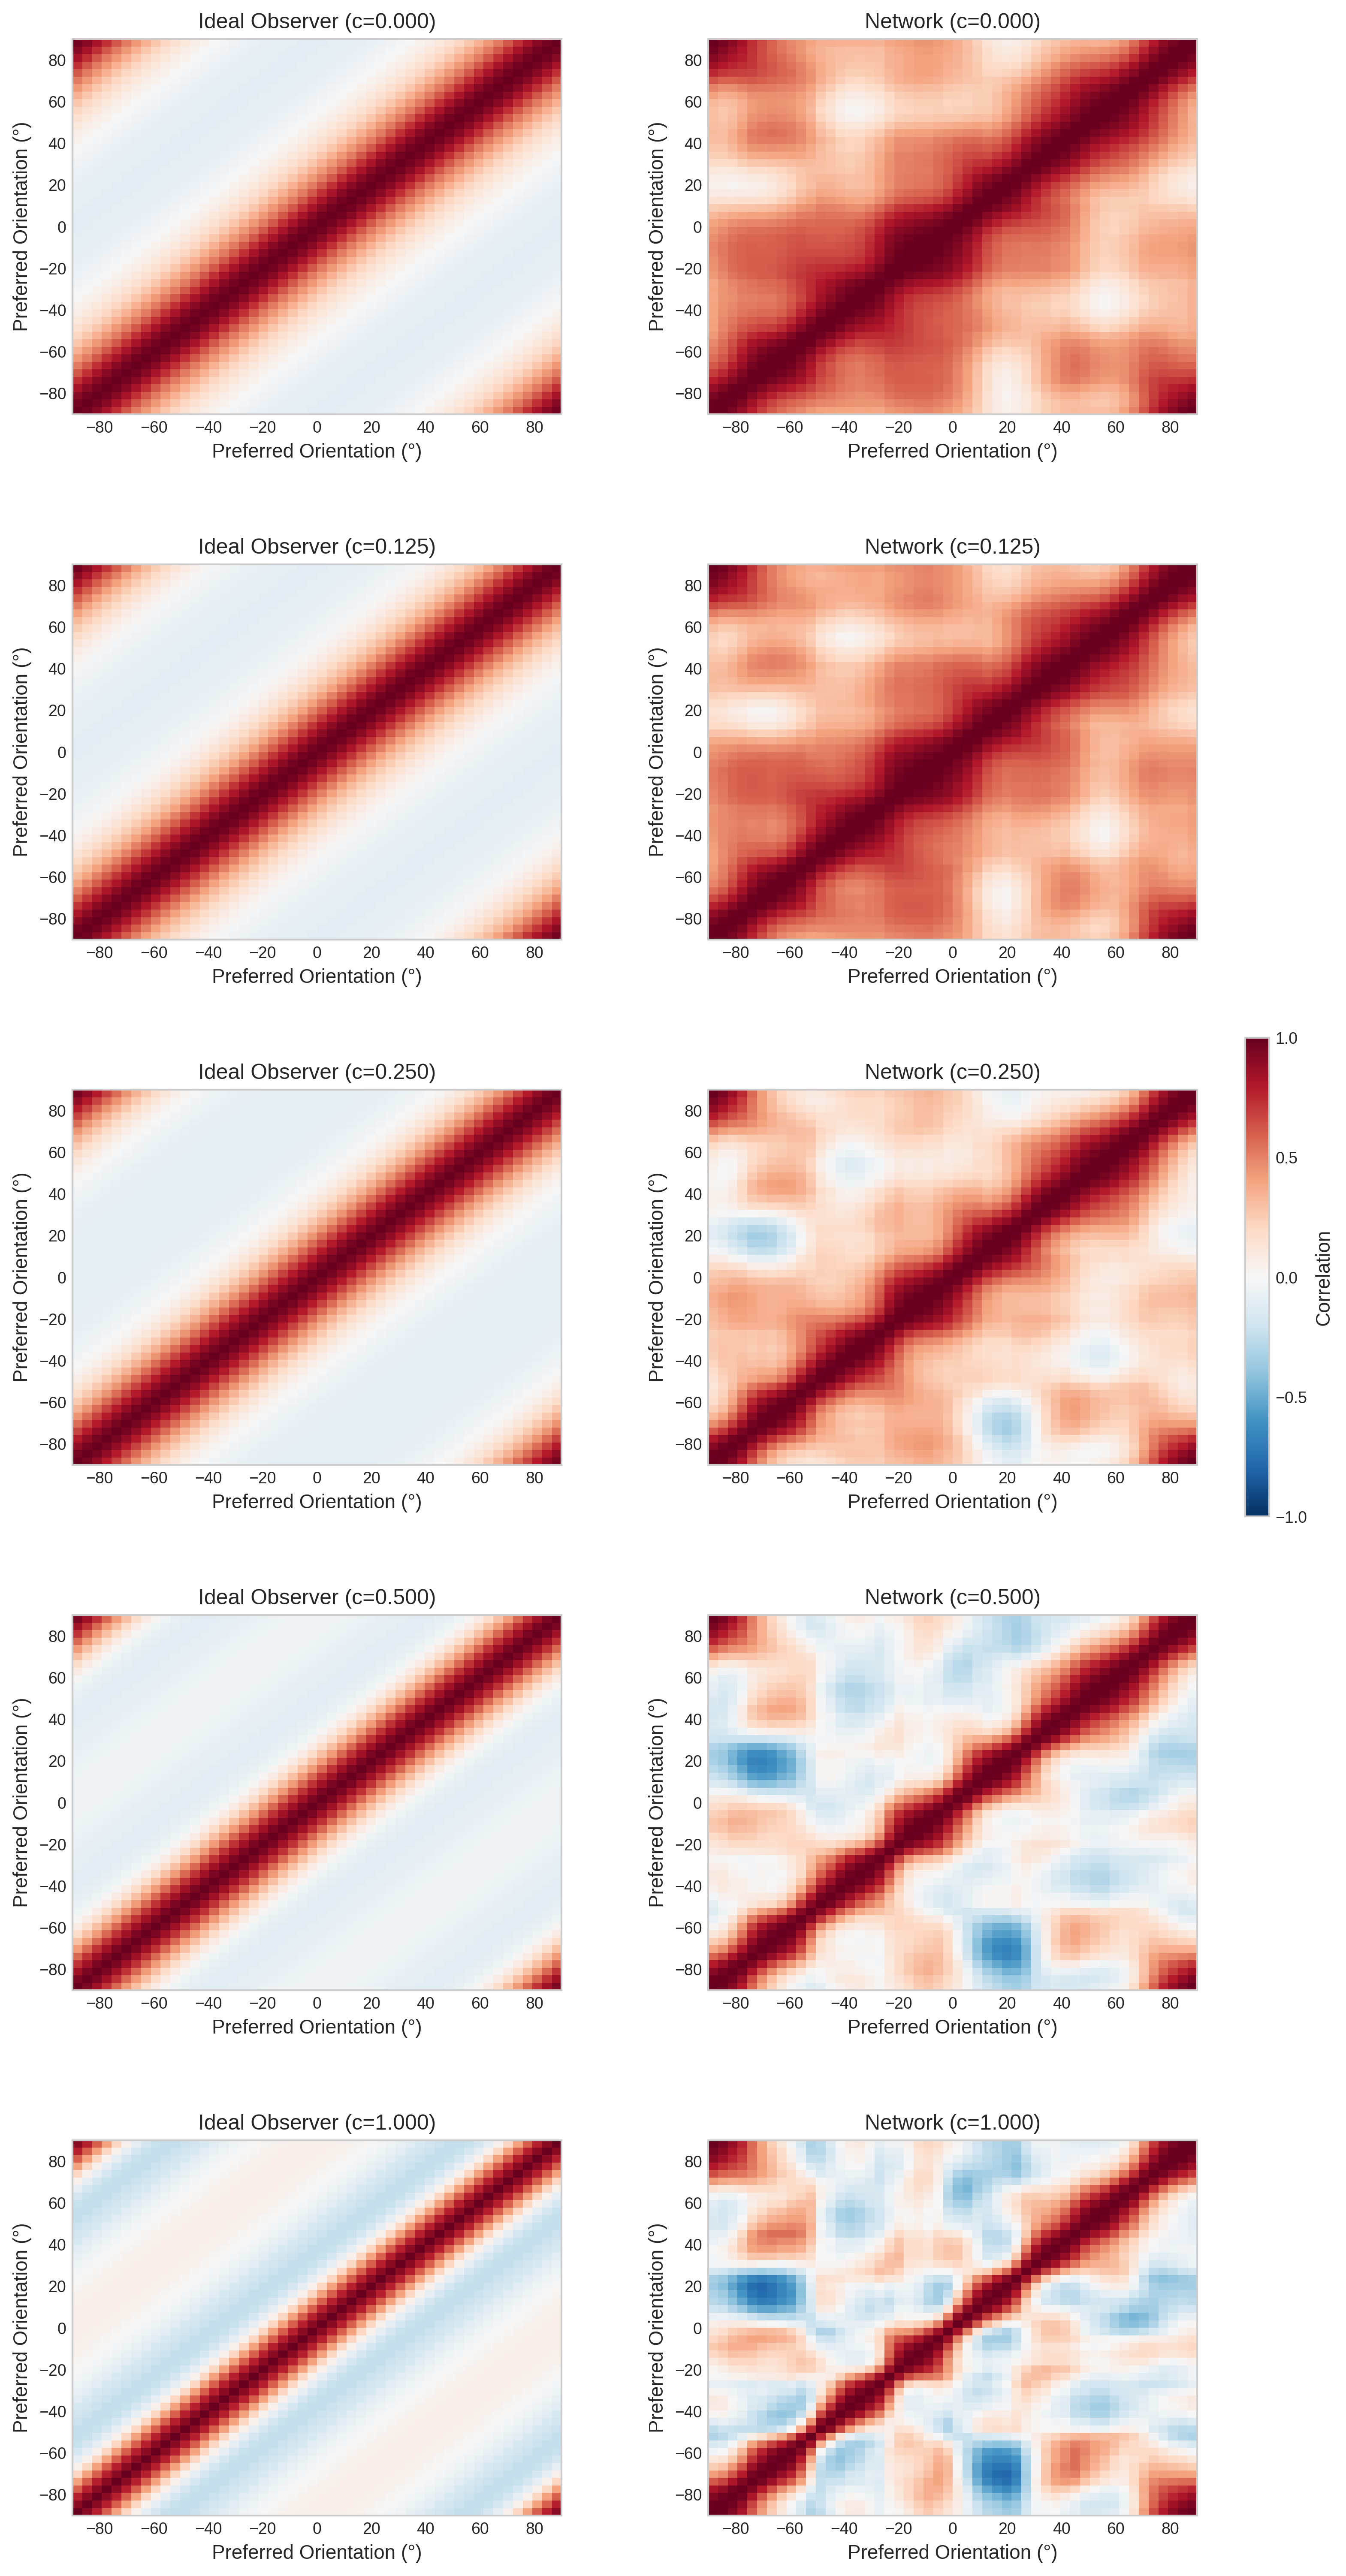
\includegraphics[width=0.6\textwidth]{08_resultados/figures/Fig2d_correlation_matrices.png}
    \caption{Matrices de correlación de Pearson entre potenciales de membrana excitatorios. Columna izquierda: observador ideal (\acrshort{GSM}). Columna derecha: red neuronal (\acrshort{SSN}). Cada columna corresponde a un nivel de contraste diferente.}
    \label{fig:fig2d}
\end{figure}


% \newgeometry{margin=0cm}
% \begin{figure}[!p]
%     \centering
%     % Imagen a página completa
%     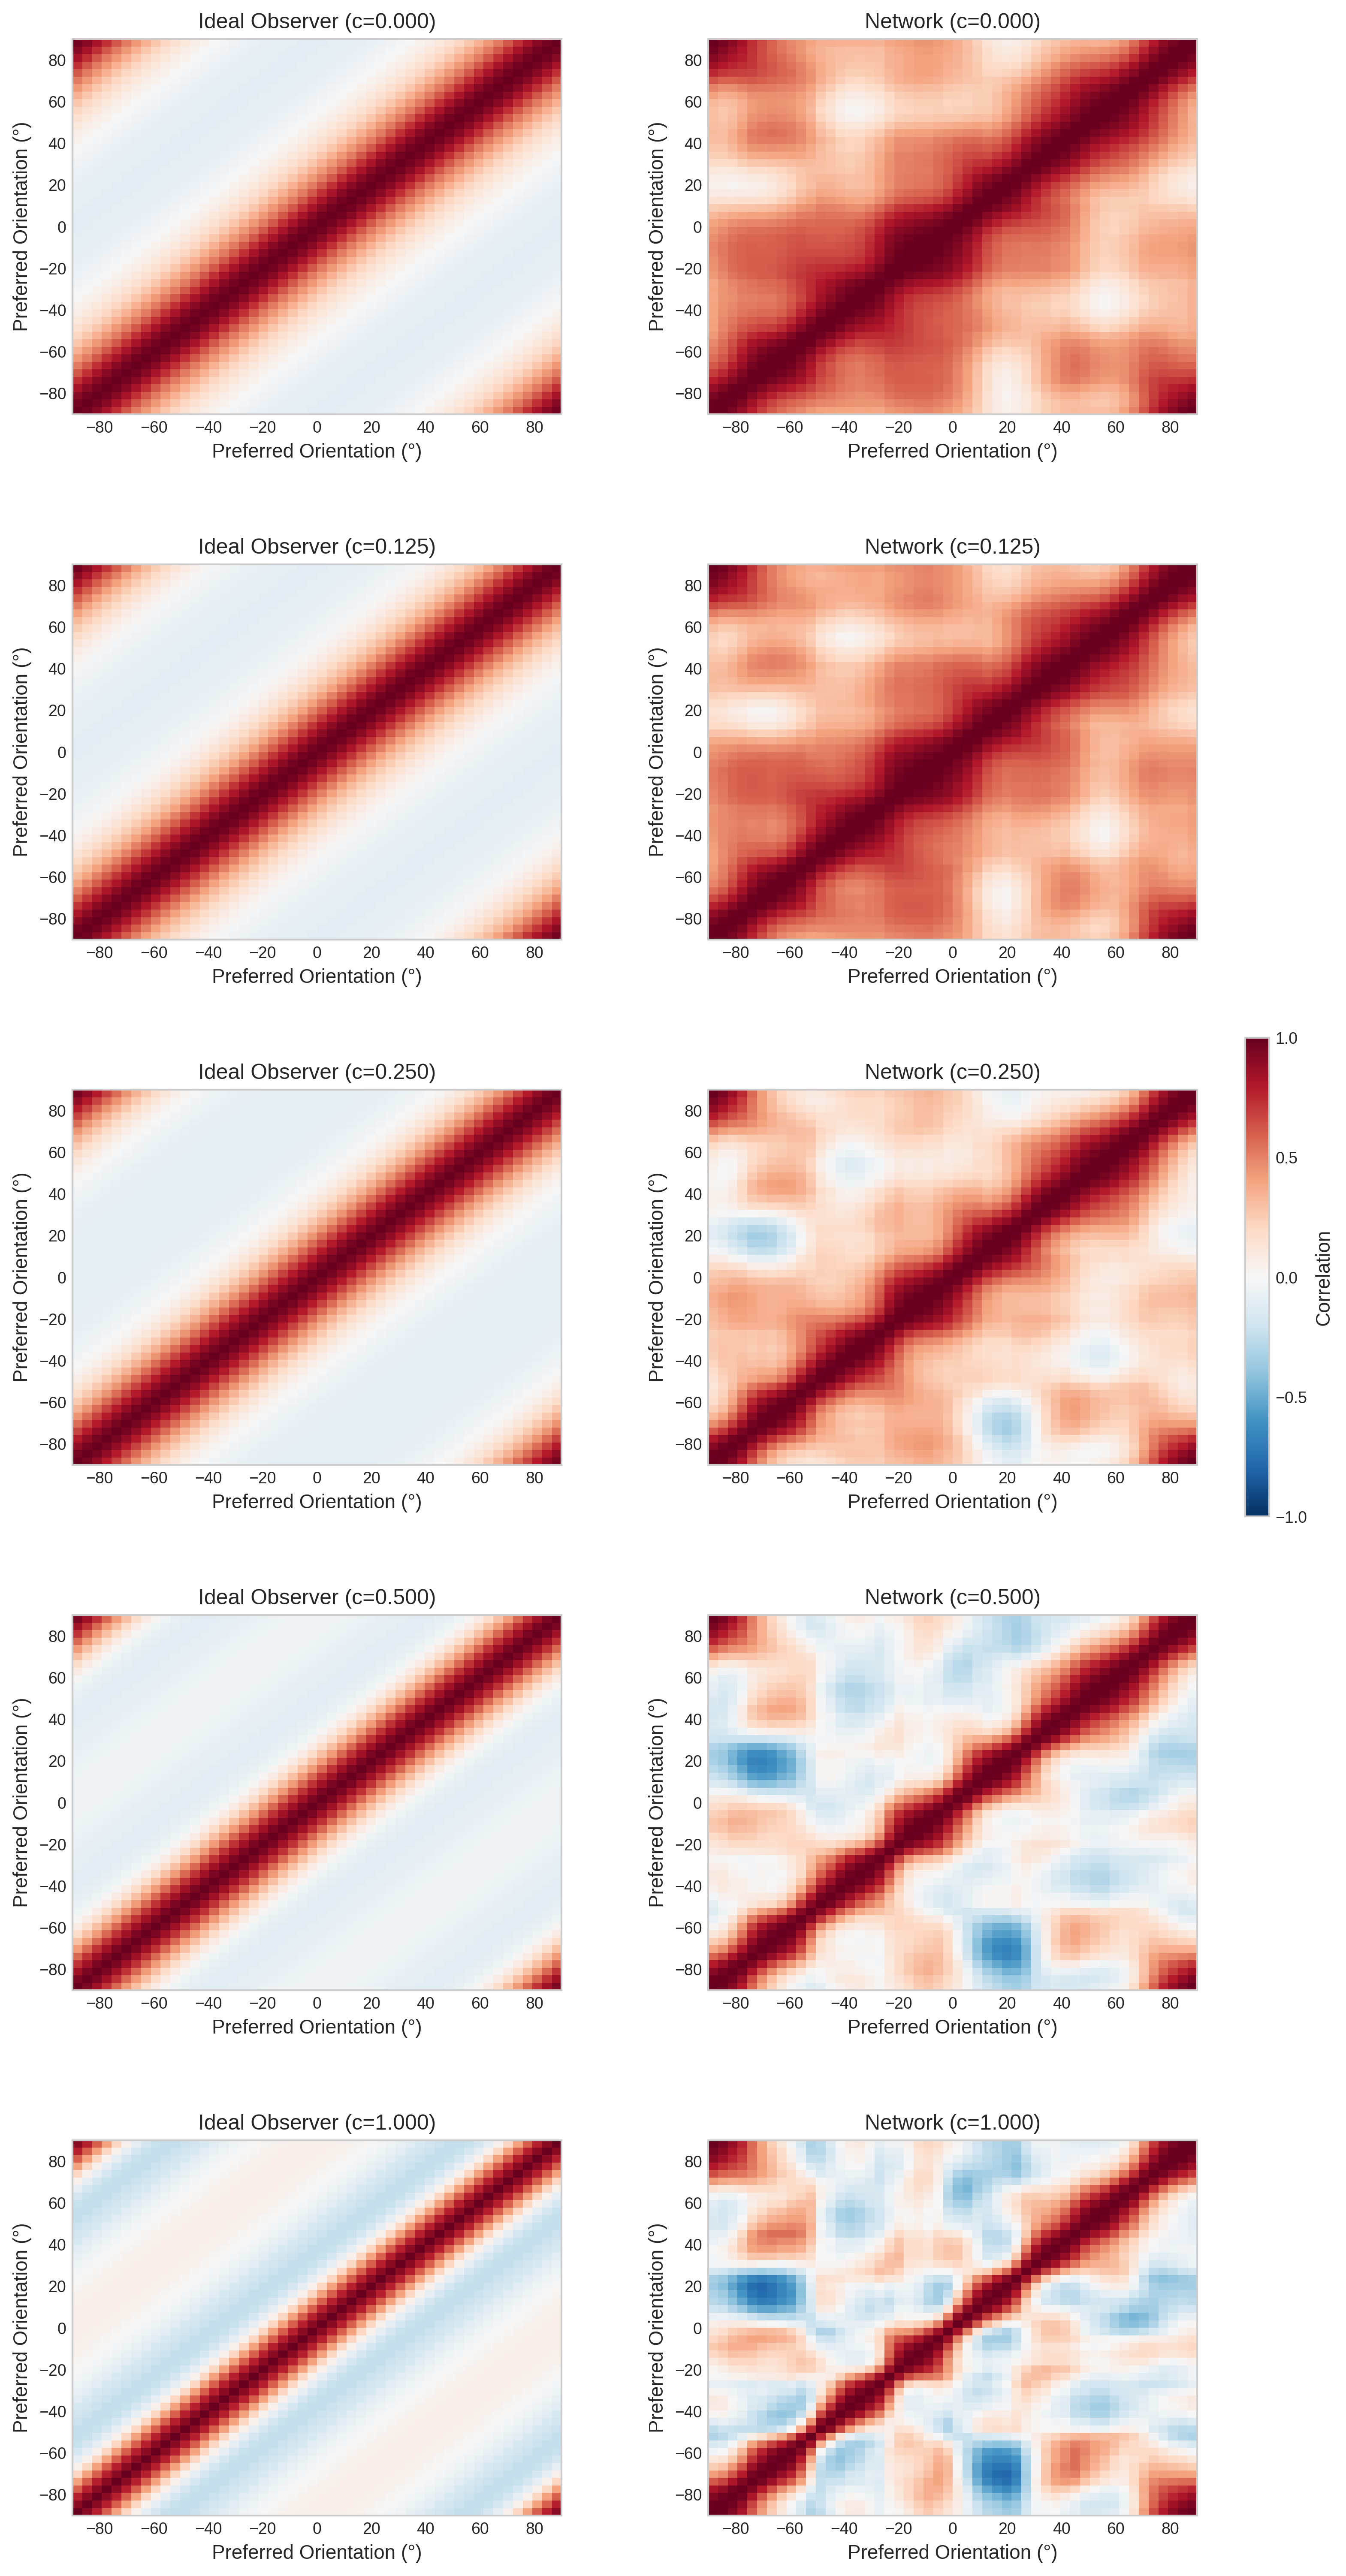
\includegraphics[height=0.8\paperheight,keepaspectratio]{08_resultados/figures/Fig2d_correlation_matrices.png}

%     % Caption limitada al ancho del texto
%     \vspace{2em}
%     \parbox{0.7\textwidth}{
%         \caption{Matrices de correlación de Pearson entre potenciales de membrana excitatorios. Columna izquierda: observador ideal (\acrshort{GSM}). Columna derecha: red neuronal (\acrshort{SSN}). Cada columna corresponde a un nivel de contraste diferente.}
%         \label{fig:fig2d}
%     }
% \end{figure}
% \restoregeometry



La diagonal principal muestra máxima correlación, y a medida que nos alejamos de la diagonal, la correlación decae gradualmente, reflejando que neuronas con orientaciones preferidas más distantes están menos correlacionadas. La estructura de correlaciones se modifica con el contraste de manera consistente entre el observador ideal y la red: para contraste cero, las correlaciones están determinadas principalmente por el prior del \acrshort{GSM}, mientras que con el aumento del contraste, la estructura refleja progresivamente más la información del estímulo. Calculando la correlación de Pearson elemento por elemento entre ambas matrices, se obtienen valores superiores a 0.95 para todos los niveles de contraste.

% =============================================================================
% SECCIÓN 4: ANÁLISIS DE PROPIEDADES DINÁMICAS
% =============================================================================

\section{Propiedades dinámicas emergentes}
\label{sec:res_dynamics}

Más allá de reproducir los momentos estadísticos correctos, el modelo de Echeveste se distingue por exhibir propiedades dinámicas que emergen como consecuencia del objetivo de muestreo sin ser explícitamente impuestas durante el entrenamiento. Esta sección presenta evidencia preliminar de que nuestra implementación preserva estas características, junto con las direcciones de trabajo futuro necesarias para una validación completa.

\subsection{Variabilidad modulada por estímulo}
\label{subsec:res_fano}

El fenómeno de quenching de variabilidad puede cuantificarse mediante el factor de Fano\footnote{El factor de Fano es una medida 
adimensional de dispersión relativa, análoga al coeficiente de variación pero apropiada para 
procesos de conteo.}, definido como $F = \text{Var}[r] / \mathbb{E}[r]$. Para un proceso de Poisson, $F = 1$; valores menores indican variabilidad sub-poissoniana, característica de respuestas corticales bajo estimulación.

El análisis cuantitativo del factor de Fano a partir de los datos de simulación muestra una reducción sistemática con el aumento del contraste: para contraste $z = 0$, el factor de Fano promedio se encuentra en el rango $1.0 - 1.2$, mientras que para $z = 1$ decrece hacia valores en el rango $0.6 - 0.8$. Esta reducción es particularmente pronunciada para las neuronas cuya orientación preferida coincide con la del estímulo, consistente con observaciones experimentales en \acrshort{V1} de primates \citep{echeveste2020cortical}.


\subsection{Análisis de oscilaciones gamma}
  \label{subsec:res_gamma}
  Una propiedad emergente notable del modelo de \citet{echeveste2020cortical} es la presencia de
  oscilaciones en el rango gamma (30-80 Hz), cuya frecuencia pico aumenta con el contraste del
  estímulo. Esta característica no es impuesta durante el entrenamiento, sino que surge como
  consecuencia de optimizar la red para realizar muestreo de la distribución posterior del
  \acrshort{GSM}. La relevancia de este hallazgo radica en que las oscilaciones gamma se observan
  consistentemente en registros electrofisiológicos de la corteza visual primaria (\acrshort{V1}) de
  primates, sugiriendo que podrían ser un subproducto funcional del cómputo probabilístico más que un
  epifenómeno.

  \subsubsection{Potencial de campo local}
  El potencial de campo local (\acrshort{LFP}) es una señal electrofisiológica que refleja la 
  actividad sináptica agregada de poblaciones neuronales en la vecindad de un electrodo de registro 
  extracelular. A diferencia de los potenciales de acción, que capturan la actividad de neuronas 
  individuales, el \acrshort{LFP} representa principalmente las corrientes sinápticas sumadas de 
  cientos a miles de neuronas, proporcionando una medida de la dinámica poblacional. En registros 
  experimentales de \acrshort{V1}, el \acrshort{LFP} exhibe oscilaciones prominentes en el rango 
  gamma durante la presentación de estímulos visuales, cuyas propiedades espectrales varían 
  sistemáticamente con parámetros del estímulo como el contraste y la orientación.

  En el contexto del modelo, el \acrshort{LFP} se aproxima como el promedio de los potenciales de 
  membrana de las neuronas excitatorias:
  \begin{equation}
      \text{LFP}(t) = \frac{1}{N_E} \sum_{i=1}^{N_E} u_E^{(i)}(t)
  \end{equation}
  Esta definición captura la actividad colectiva de la población excitatoria, constituyendo un 
  análogo computacional de la señal medida experimentalmente. La elección de promediar únicamente 
  sobre neuronas excitatorias sigue la convención del trabajo original y refleja que las neuronas 
  piramidales (excitatorias) contribuyen predominantemente al \acrshort{LFP} debido a su geometría 
  dendrítica extendida.


  \subsubsection{Análisis espectral}
 Para caracterizar el contenido oscilatorio del \acrshort{LFP}, se calculó su espectro de potencia, 
que describe cómo se distribuye la energía de la señal entre sus diferentes componentes 
frecuenciales. Una señal con oscilaciones gamma prominentes exhibirá un pico en el espectro 
dentro del rango 30-80 Hz.

La estimación espectral se realizó mediante el método de Welch, una técnica estándar en el 
análisis de señales neurofisiológicas. Este método divide la señal temporal en segmentos 
superpuestos, calcula el espectro de cada segmento individualmente, y promedia los resultados. 
El promediado reduce la variabilidad del estimador a costa de cierta pérdida en resolución 
frecuencial, proporcionando estimaciones más estables que las obtenidas a partir de la señal 
completa. En nuestro análisis, se utilizaron ventanas de Hanning con 50\% de solapamiento, 
parámetros comúnmente empleados en estudios de \acrshort{LFP} cortical.

La frecuencia pico gamma se identificó como el máximo del espectro dentro del rango 30-80 Hz 
para cada condición de contraste.

  \subsubsection{Resultados}
  La Figura~\ref{fig:gamma_analysis} presenta los resultados del análisis espectral para los cinco 
  niveles de contraste del conjunto de entrenamiento. Los paneles individuales muestran el espectro 
  de potencia en escala logarítmica, donde la banda sombreada indica el rango gamma (30-80 Hz) y las
  líneas punteadas marcan la frecuencia pico detectada dentro de este rango. El panel inferior 
  derecho sintetiza el resultado principal: la frecuencia pico gamma en función del contraste.
  \begin{figure}[!ht]
      \centering
      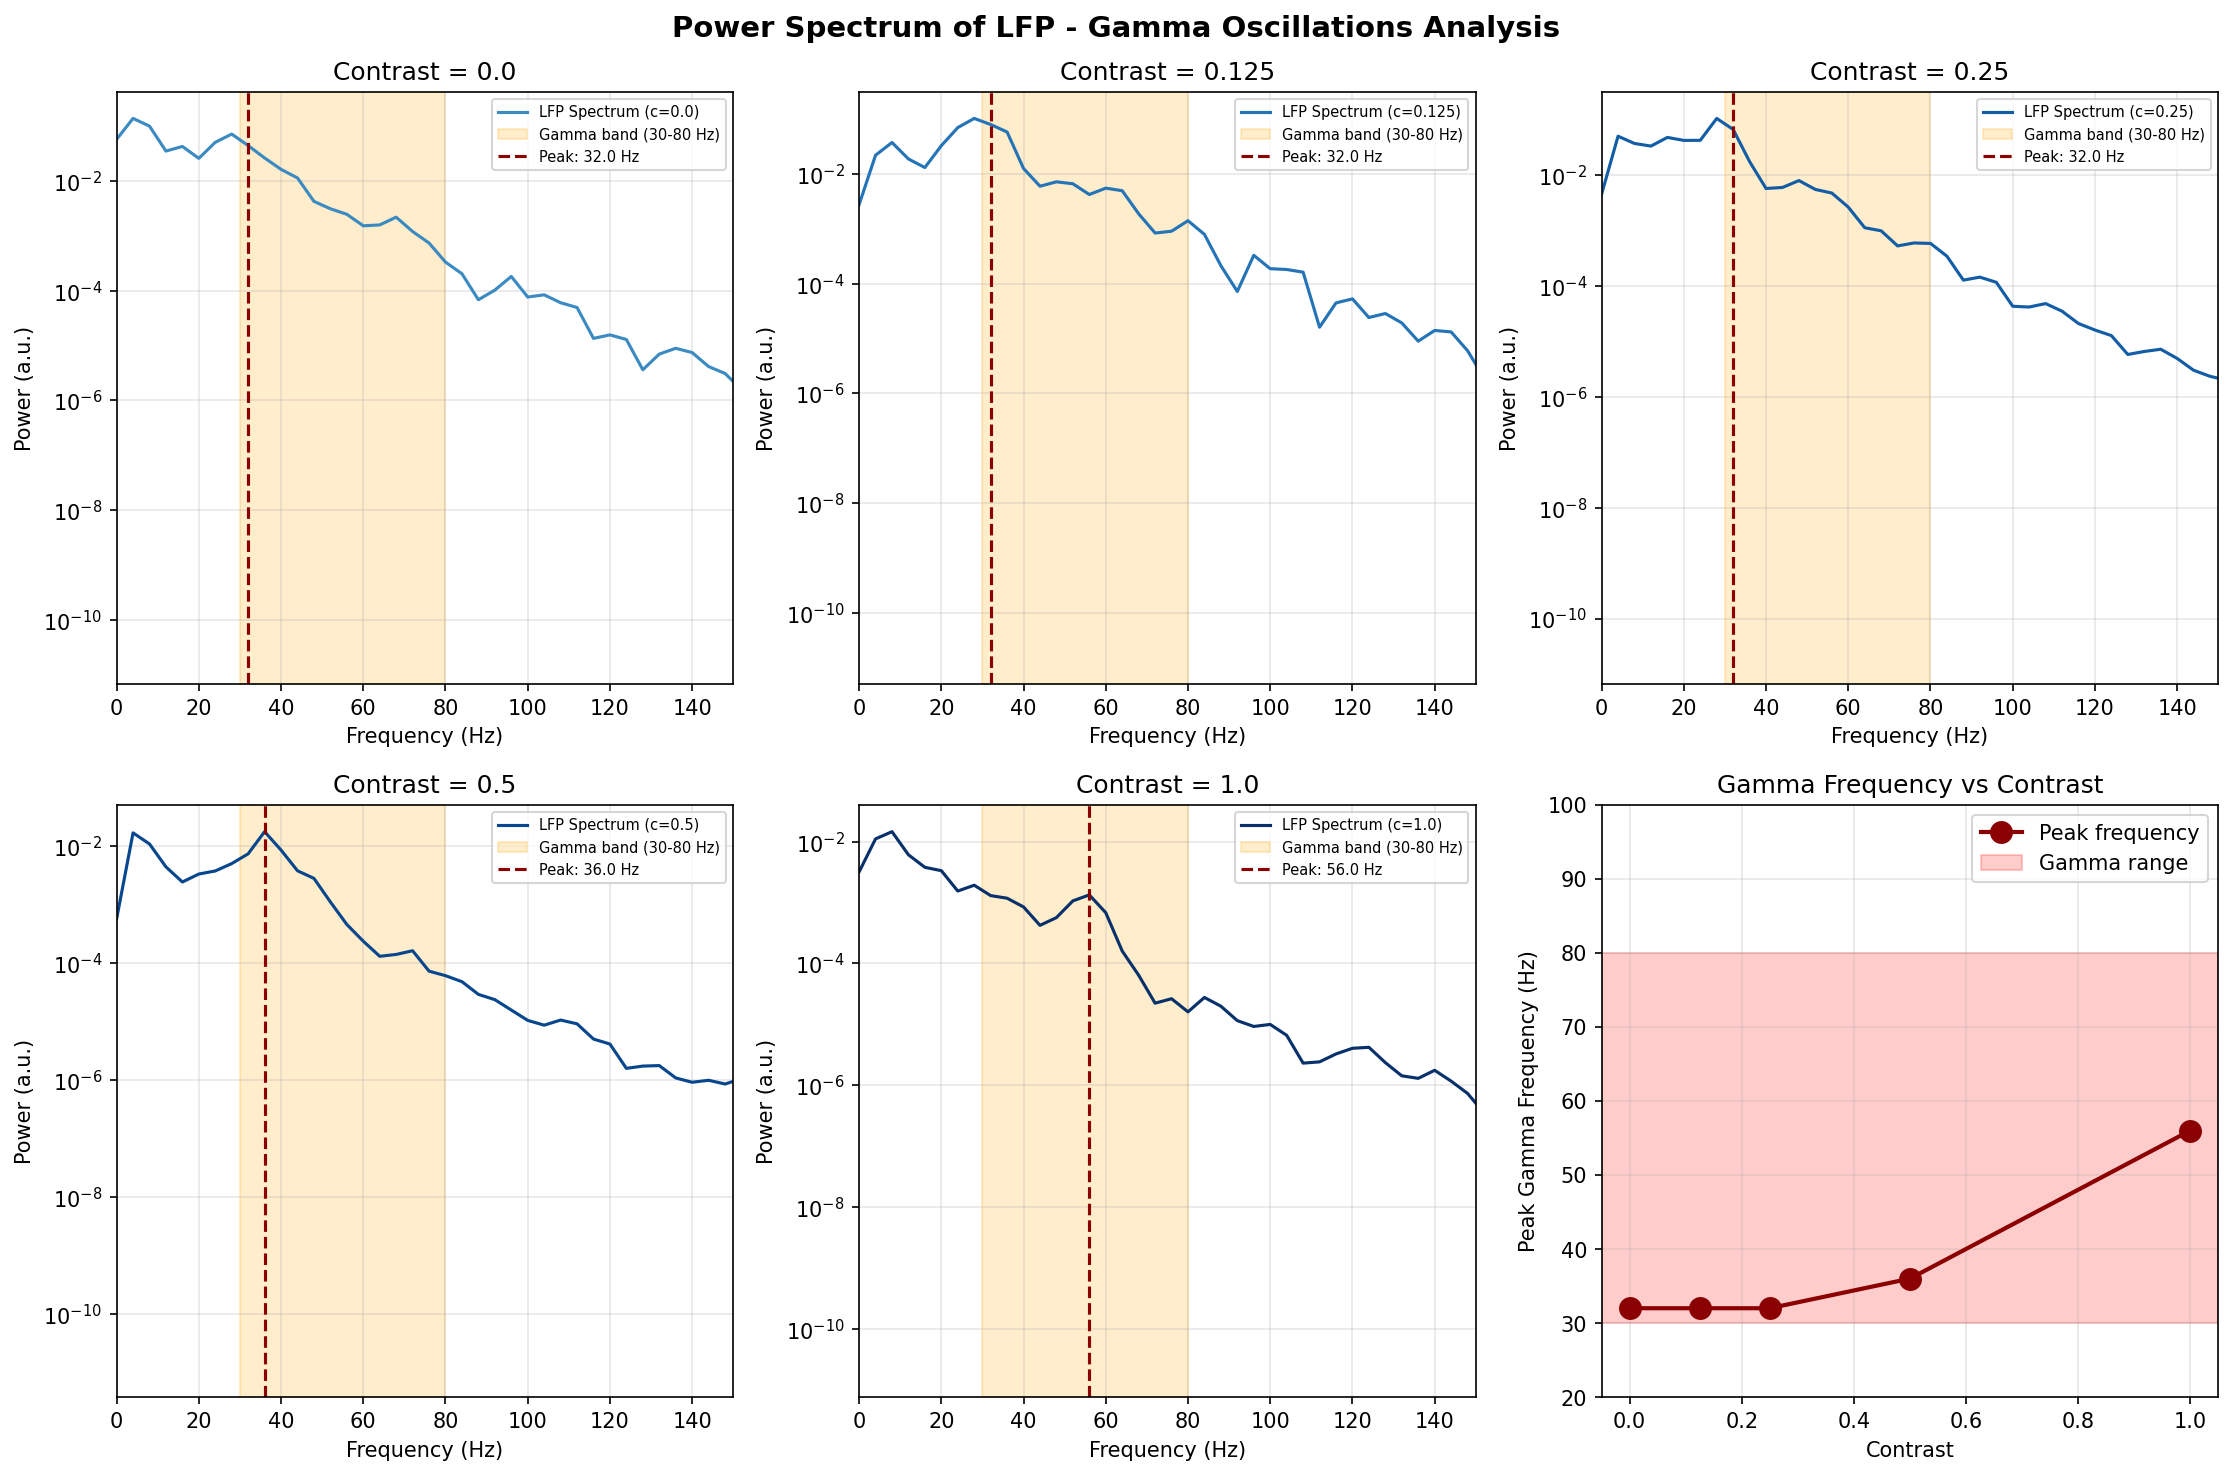
\includegraphics[width=0.95\textwidth]{08_resultados/figures/gamma_oscillations_analysis.png}
      \caption{Análisis espectral del potencial de campo local (\acrshort{LFP}). Los cinco primeros 
      paneles muestran el espectro de potencia para cada nivel de contraste, con la banda gamma 
      (30-80 Hz) sombreada en rojo y la frecuencia pico indicada con línea punteada. El panel 
      inferior derecho muestra la dependencia de la frecuencia pico con el contraste, confirmando 
      el incremento predicho por el modelo: de aproximadamente 32 Hz (contraste bajo) a 56 Hz 
      (contraste máximo).}
      \label{fig:gamma_analysis}
  \end{figure}
  Los resultados confirman que la red implementada reproduce la fenomenología reportada en el 
  artículo original. Para contraste nulo o bajo ($z \leq 0.25$), la frecuencia pico se mantiene 
  alrededor de 32 Hz, correspondiente al extremo inferior del rango gamma. A medida que el contraste 
  aumenta, la frecuencia pico se desplaza progresivamente hacia valores más altos, alcanzando 
  aproximadamente 56 Hz para contraste máximo ($z = 1.0$). Este comportamiento es cualitativamente 
  consistente con observaciones experimentales en \acrshort{V1}, donde se ha reportado que la 
  frecuencia de oscilaciones gamma aumenta con el contraste del estímulo visual 
  \citep{echeveste2020cortical}.

  Desde una perspectiva computacional, este fenómeno puede interpretarse en términos de la dinámica 
  de muestreo: mayor contraste implica mayor certeza sobre el estímulo (menor varianza posterior), 
  lo que permite a la red explorar el espacio de estados más rápidamente, manifestándose como 
  oscilaciones de mayor frecuencia. Esta interpretación conecta las propiedades espectrales 
  observadas con la función de inferencia probabilística que la red implementa.

% \subsection{Transitorios al inicio del estímulo}
% \label{subsec:res_transients}

% Los overshoots transitorios al inicio del estímulo representan otra propiedad emergente del modelo que cumple un rol funcional en la reducción del tiempo de burn-in para la inferencia. Simulaciones preliminares utilizando el modo \texttt{three\_phase} muestran indicios de respuestas transitorias consistentes con las predicciones teóricas.

% \subsection{Validaciones pendientes}
% \label{subsec:res_pending}

% Para completar la validación según los estándares establecidos por \citet{echeveste2020cortical}, se identifican las siguientes direcciones de trabajo futuro:

% \textbf{Pruebas de generalización} (Figura 3 del artículo original): verificación de que la red interpola correctamente a niveles de contraste no entrenados, y evaluación del rendimiento con un conjunto de 500 estímulos nuevos generados por el \acrshort{GSM} que incluyen múltiples orientaciones dominantes.

% \textbf{Análisis espectral completo}: verificación de oscilaciones gamma mediante análisis de potencia espectral del potencial de campo local (\acrshort{LFP}), incluyendo la dependencia de la frecuencia pico con el contraste.

% \textbf{Redes de control}: el artículo original entrena múltiples redes que difieren en un único aspecto (sin modulación de covarianza, sin principio de Dale, sin penalización de slowness, con factores de Fano constantes), demostrando la necesidad de cada componente. La implementación de estas comparaciones constituye una validación importante.

% \textbf{Comparación con datos experimentales} (Figura 7): validación de que las propiedades de la red optimizada son consistentes con registros electrofisiológicos de \acrshort{V1} en primates.

% =============================================================================
% SECCIÓN 5: RESUMEN
% =============================================================================

\section{Resumen del capítulo}
\label{sec:res_summary}

Este capítulo presentó los resultados de la validación de nuestra implementación del modelo de \citet{echeveste2020cortical} en múltiples niveles. La validación función por función demostró equivalencia numérica exacta con errores del orden de la precisión de punto flotante ($\sim 10^{-15}$). Las pruebas unitarias verificaron la correctitud de componentes individuales. El procedimiento de entrenamiento demostró convergencia robusta hacia parámetros comparables a los de referencia. Las simulaciones replicaron las figuras centrales del artículo original, confirmando que la red implementa correctamente muestreo de la distribución posterior del modelo generativo \acrshort{GSM}.

Estos resultados establecen que la implementación está lista para su uso en investigaciones que requieran un modelo de dinámicas corticales biológicamente realistas para inferencia probabilística unimodal. Las validaciones pendientes identificadas, particularmente respecto a generalización, análisis espectral y redes de control, definen direcciones claras para trabajo futuro.